\chapter{Sistemas autónomos}


En esta unidad abordaremos el estudio de  sistemas no lineales y
autónomos, en particular sistemas autónomos planos.
\section{Ecuaciones autónomas}

Una ecuación
\begin{equation}\label{ecuaaut}
    x'(t)=f(x(t)),
\end{equation}
donde $\Omega$ es un subconjunto abierto de $\mathbb{R}^n$ y $
f:\Omega\to\mathbb{R}^n$, se denomina \emph{ecuación autónoma}. De
ahora en más asumiremos que $f$ es de clase $C^1$ en $\Omega$, de
modo que para cada $(t_0,x^0)\in\rr\times\Omega$ existe una
solución $\varphi(t)$ que pasa por $(t_0,x^0)$. Cuando invoquemos
esta solución supondremos que es una solución máxima y denotaremos
su intervalo de definición por
$I_{\varphi}=(a_{\varphi},b_{\varphi})$. Las soluciones a
ecuaciones autónomas tienen la siguiente  propiedad.

\begin{teorema}{invartras} Si $\varphi$ es solución de \eqref{ecuaaut}
entonces $\psi(t)=\varphi(t+c)$ es también solución e
$I_{\psi}=I_{\varphi}-c$.
\end{teorema}
\begin{demo} Por la regla de la cadena y \eqref{ecuaaut}
\[
    \psi'(t)=\varphi'(t+c)=f(\varphi'(t+c))=f(\psi'(t)).
\]
\end{demo}
Vemos así que toda trasladada, sobre el eje $t$, de una solución
es también solución. Si $x^0\in\Omega$ satisface que $f(x^0)=0$
entonces $\varphi(t)\equiv x^0$ es una solución. Dado que esta solución
no experimenta cambios con el tiempo, $x^0$ se denomina
\emph{punto de equilibrio} del sistema \eqref{ecuaaut}. El teorema
anterior tiene la siguiente consecuencia.

\begin{teorema}{orbitasnoencuentran} Si $\varphi$ y $\psi$ son soluciones de
\eqref{ecuaaut} y $\varphi(t_0)=\psi(t_1)$ entonces existe un $c\in\rr$
tal que $\varphi(t)=\psi(t+c)$.
\end{teorema}
\begin{demo} Por el Teorema \ref{invartras}, la función
$\psi_1(t):=\psi(t+t_1-t_0)$ es solución y, por hipótesis,
$\psi_1(t_0)=\varphi(t_0)$, así, por unicidad, $\varphi(t)=\psi_1(t)$ para
todo $t$. \end{demo}

\begin{corolario}{} Si $\varphi$ es solución de \eqref{ecuaaut} y
$\varphi(t_0)=\varphi(t_1)$ para ciertos $t_0\neq t_1$ entonces $\varphi$ es
periódica.
\end{corolario}
\begin{demo} Por el teorema anterior aplicado a $\psi=\varphi$
obtenemos $\varphi(t)=\varphi(t+c)$, luego $\varphi$ es periódica.\end{demo}


\section{Ecuaciones unidimensionales}

\begin{ejemplo}{}Considerar la ecuación
\[
    x'=x,\quad x\in\rr,
\]
que tiene por solución general $\varphi(t)=Ce^t$. Notar que el conjunto
$\Omega$, en este caso $\Omega=\rr$, queda dividido en tres
regiones $(-\infty,0)$, $\{0\}$ y $(0,\infty)$. Cada una de estas
tres regiones es imagen de soluciones, por ejemplo $(0,+\infty)$
es imagen de las soluciones positivas. Notar que hay una cantidad
infinita de soluciones positivas, de hecho está la solución
$\varphi_0(t)=e^t$ y todas sus trasladadas.

\begin{figure}[h]
\begin{center}
\def\Func{ neg }
 %
\psset{method=rk4,linecolor=blue,linewidth=0.5pt,unit=.5cm}
\begin{pspicture}(-5,-5)(5,5)
    \begin{psclip}{\psframe[linecolor=black](-5,-5)(5,5)}
\multido{\r=-5+1}{11}{
  \psplotDiffEqn[arrows=>-,arrowscale=2]{\r}{5}{1}{\Func}
    \psplotDiffEqn{\r}{-5}{1}{\Func}
} \multido{\r=-5+1}{11}{
  \psplotDiffEqn[arrows=>-,arrowscale=2]{\r}{5}{-1}{\Func}
    \psplotDiffEqn{\r}{-5}{-1}{\Func}
}
 \psplotDiffEqn[arrows=>-,arrowscale=2]{0}{5}{0}{\Func}
    \psplotDiffEqn{0}{-5}{0}{\Func}
\end{psclip}
\end{pspicture}

\end{center}
\caption{Ecuación $x'=x$}\label{ecuaexp}
\end{figure}

El conjunto $\{0\}$ es la imagen de la función nula, que,
obviamente, coincide con sus trasladadas. Notar que $0$ es un
punto de equilibrio.

\end{ejemplo}


\begin{ejemplo}{} Consideremos ahora
\[
    x'=\frac12(x^2-1).
\]
Para resolver esta ecuación escribamos
\[
    dt=\frac{2dx}{x^2-1}
\]
e integremos
\[
\begin{split}
    t+c=\int \frac{2dx}{x^2-1}&=\int\frac1{x-2}-\frac1{x+1}dx\\
                               &=\ln\bigg|\frac{x-1}{x+1}\bigg|.
\end{split}
\]
Luego
\[
    x(t)=\frac{1\pm ke^t}{1\mp ke^t},\quad k>0
\]
es la  solución general. Notar que hay dos ``ramas'' de $x(t)$ que
corresponden a los intervalos $(-\infty,-\ln k)$ y $(-\ln
k,+\infty)$. En realidad hay que pensar estas ramas como dos
soluciones máximas diferentes. La primera tiene su gráfica debajo
de $-1$ y la segunda por encima de $1$. Las soluciones que
empiezan en $(-1,1)$ están definidas en todo $\rr$ y permanecen en
$(-1,1)$. Los puntos $-1$ y $1$ son de equilibrio de la ecuación.

\begin{figure}[h]
\begin{center}
\def\Funct{(y[0]^2-1)/2 }
 %
\psset{method=rk4,linecolor=blue,linewidth=0.5pt,unit=.5cm}
\begin{pspicture}(-5,-5)(5,5)
    \begin{psclip}{\psframe[linecolor=black](-5,-5)(5,5)}
\multido{\r=-5+1}{10}{
  \psplotDiffEqn[arrows=>-,arrowscale=2,algebraic=true]{\r}{5}{.5}{\Funct}
  \psplotDiffEqn[algebraic=true]{\r}{-5}{.5}{\Funct}
  }
\multido{\r=-5+1}{10}{
  \psplotDiffEqn[algebraic=true]{\r}{-5}{5}{\Funct}
  }
\multido{\r=-5+1}{10}{
  \psplotDiffEqn[algebraic=true]{\r}{5}{-5}{\Funct}
  }

\end{psclip}
\end{pspicture}
\end{center}
\caption{Ecuación $x'=\frac12(x^2-1)$}\label{fig2}
\end{figure}

Como muestra la figura \ref{fig2}, ahora tenemos dividido
$\Omega=\rr$ en cinco regiones $(-\infty,-1)$, $\{-1\}$, $(-1,1)$,
$\{1\}$ y $(1,+\infty)$. Las propiedades cualitativas de cualquier
solución en cualquiera de estas ramas son determinadas por las de
cualquier solución fija en una de estas ramas, ya que una es una
trasladada de la otra. Notar que si $x(t_0)$ no es un punto de
equilibrio entonces $x'(t)=f(x(t))\neq 0$ para todo $t$, luego
$x(t)$ es una función monótona. Por ende, si $x$ está definida en
un intervalo $(a,+\infty)$ el siguiente límite
$x^0:=\lim_{t\to+\infty}x(t)$ debe existir. Si $x^0\in\rr$
entonces, por el ejercicio \ref{ejerptoequi}, debe ser un punto de
equilibrio, de lo contrario $x^0=\pm\infty$. Notar que, como toda
solución máxima $\varphi(t)$ satisface que $(t,\varphi(t))$ se sale de
cualquier compacto contenido en $\rr\times\Omega$, se tiene que si
$\varphi(t_0)$ está entre dos puntos de equilibrio, $\varphi(t)$ permanece
entre ellos para todo tiempo e $I_{\varphi}=\rr$.  En el ejemplo, como
$f(x)<0$ en $(-1,1)$ debemos tener que una solución $\varphi$ tal que
$\varphi(t_0)\in (-1,1)$ está definida en $\rr$ y
$1=\lim_{t\to-\infty}\varphi(t)$ y $-1=\lim_{t\to +\infty}\varphi(t)$. Toda
esta información cualitativa la podemos representar en el eje $x$
como en la figura \ref{retrato1}. Las flechas indican la dirección
en que las soluciones recorren la región. Este tipo de
representación la llamaremos \emph{retrato de fases}

\begin{figure}[h]
\begin{center}
\psset{unit=1mm}  \pspicture(0,0)(100,30)
    \psline(0,15)(100,15)
    \pscircle*(30,15){1}
    \pscircle*(70,15){1}
    \psline{->}(0,15)(15,15)
    \psline{->}(70,15)(45,15)
    \psline{->}(70,15)(85,15)
    \rput(29,18){$-1$}
     \rput(69,18){$1$}
     \rput(100,18){$x$}
 \endpspicture
\end{center}
\caption{Retrato de fases de $x'=\frac12(x^2-1)$.}\label{retrato1}
\end{figure}
\end{ejemplo}

Se observa que de haber una cantidad finita de puntos de
equilibrio hay sólo una cantidad finita posible de retratos de
fases. Por ejemplo si hay sólo un punto de equilibrio hay sólo los
cuatro retratos de fases mostrados en la figura \ref{retrato2}.
Por ejemplo $x'=x$, $x'=x^3$ y $x'=x-a$, tienen el mismo retrato
de fases d). En este caso diremos que las tres ecuaciones son
\emph{cualitativamente equivalentes}.

\begin{figure}[h]
\begin{center}
\psset{unit=1mm}  \pspicture(0,0)(100,30)

    \rput(-3,25){a)}
    \psline(0,25)(30,25)
    \pscircle*(15,25){1}

    \psline{->}(0,25)(7,25)
    \psline{->}(30,25)(22.5,25)
    \rput(50,0){
    \rput(-3,25){b)}
    \psline(0,25)(30,25)
    \pscircle*(15,25){1}

    \psline{->}(0,25)(7,25)
    \psline{->}(15,25)(22.5,25)
} \rput(0,-10){    \rput(-3,25){c)}
    \psline(0,25)(30,25)
    \pscircle*(15,25){1}

    \psline{<-}(7,25)(15,25)
    \psline{->}(30,25)(22.5,25)
    \rput(50,0){
    \rput(-3,25){d)}
    \psline(0,25)(30,25)
    \pscircle*(15,25){1}

    \psline{->}(15,25)(22.5,25)
    \psline{->}(15,25)(7,25)
}}


    \endpspicture
\end{center}
\caption{Retrato de fases un punto de equilibrio}\label{retrato2}
\end{figure}



\section{Sistemas autónomos planos}
Ahora consideraremos la ecuación
\begin{equation}\label{sisautplano}
    x'=f(x),\quad f:\Omega\to\rr^2,
\end{equation}
donde $\Omega$ es un abierto de $\rr^2$.  En un sistema autónomo
unidimensional el retrato de fases queda completamente determinado
por la cantidad de puntos de equilibrio
 y el comportamiento de las soluciones cerca de sus puntos
de equilibrio, esto, a la vez, determina las propiedades
cualitativas de las soluciones. En otras palabras, estudiando
propiedades locales, cerca de los puntos de equilibrio, de las
soluciones inferimos su comportamiento cualitativo global. En
dimensiones mayores las propiedades cualitativas de las soluciones
de ecuaciones no lineales  no se pueden analizar sólo a partir de
propiedades locales. Es por ello que el análisis de sistemas
autónomos planos implica desarrollar dos teorías: una local y otra
global.

\subsection{Técnicas elementales}

Como en el caso de un sistema unidimensional, las soluciones de
\ref{sisautplano} determinarán regiones de $\Omega$. Como
consecuencia del Teorema \ref{orbitasnoencuentran} obtenemos que
estas regiones son disjuntas. Cada una de ellas es la imagen de
alguna solución $\varphi$, y por ende también de cualquier trasladada
de $\varphi$. En símbolos estas regiones son los conjuntos
$\varphi(I_{\varphi})$, con $\varphi$ solución. Es por ello que estas regiones
son curvas de $\rr^2$ y nos referiremos a ellas como
\emph{trayectorias} u \emph{órbitas}\index{orbitas@órbitas} de
\eqref{sisautplano}. Algunas veces es relativamente  sencillo
construir estas órbitas por técnicas elementales. Estas técnicas
incluyen
\begin{enumerate}
    \item Estudiar las simetrías de la ecuación.
    \item Distinguir si el sistema está desacoplado.
    \item Eliminar el tiempo de la ecuación.
    \item Transformar el sistema por un cambio de variables.
\end{enumerate}
 En los siguientes ejemplos ilustramos estas técnicas.





\begin{ejemplo}{}\textbf{Ecuación del péndulo.} Consideremos la ecuación del péndulo plano
\begin{equation}\label{ecuapend}
\left\{%
\begin{array}{l}
    x_1'=x_2 \\
    x_2'=-\sen(x_1) \\
\end{array}%
\right.
\end{equation}
Para construir las trayectorias de \eqref{ecuapend} vamos usar una
técnica que consiste en eliminar el tiempo de la ecuación y
relacionar a $x_2$ con $x_1$ por medio de una ecuación, a saber:
\[
    \frac{dx_2}{dx_1}=\frac{-\sen(x_1)}{x_2 }.
\]
Resolviendo esta ecuación con variables separadas obtenemos
\[
    x_2=\pm\sqrt{2\cos(x_1)+c}.
\]
Para que esta ecuación tenga solución debemos tener $c\geq -2$.
Notar que los puntos de equilibrio del sistema son los puntos
$(n\pi,0)$, con $n\in\mathbb{Z}$. Si $(x_1,x_2)$ resuelve
\eqref{ecuapend} entonces $(-x_1,-x_2)$ también lo hace, de modo
que es suficiente obtener las trayectorias para $x_2\geq 0$ las
trayectorias por debajo del eje $x_1$ se obtienen reflejando las
de arriba respecto al origen (observar que esta reflexión puede
invertir el recorrido de las trayectorias). Así supongamos que
\[
    x_2=\sqrt{2\cos(x_1)+c}.
\]
Observar que $x_1'=x_2>0$ de modo que $x_1$ crece en el semiplano
superior y, por ende, las trayectorias se recorren de izquierda a
derecha en el semiplano superior. En el semiplano inferior el
sentido es pues de derecha a izquierda. Si $c>2$ entonces $x_2>0$
para todo $t$ e $x_2$ es una función periódica de $x_1$ con
mínimos en $2n\pi$, $n\in\mathbb{Z}$, y máximos en $(2n+1)\pi$,
$n\in\mathbb{Z}$. Si $c=2$ la trayectoria va desde $(-\pi,0)$ a
$(\pi,0)$ (lo mismo ocurre en cada intervalo que resulta de
trasladar el intervalo $(-\pi,\pi)$ por un múltiplo de $2\pi$), no
obstante estas trayectorias no puede tocar a los puntos de la
forma $((2n+1)\pi,0)$ ya que las trayectorias son disjuntas. Vemos
así que estas últimas trayectorias se realizan en un tiempo
infinito. Si $-2<c<2$ la parte de la trayectoria donde $x_2\geq 0$
y $-\pi <x_1<\pi$ va desde el punto $(-\xi,0)$ a $(\xi,0)$, con
$\cos(\xi)=-\frac{c}{2}$. Esta trayectoria se ``empalma'' con su
reflejada que irá en el sentido contrario de modo que estas
trayectorias provienen de soluciones periódicas. Por otro lado es
fácil verificar que
\[
    \|Df\|=\bigg\|\begin{pmatrix}
    0&1\\-\cos(x_1)&0\end{pmatrix}\bigg\|= 1,
\]
luego $f=(f_1,f_2)$ es lipchistziana sobre $\rr^2$ y las
soluciones están definidas para todo tiempo. El aspecto del
retrato de fases es mostrado en la figura \ref{pendulo}.
\begin{figure}[h]
\begin{center}
\def\Func{y[1]|-sin(y[0])}
\psset{xunit=.7cm,yunit=1cm,algebraic=true,linewidth=0.5pt}

\begin {pspicture}(-3.14,-3)(6.28,3)


\psset{method=rk4,plotpoints=400,linecolor=blue,linewidth=1pt,
   whichabs=0,whichord=1}

\begin{psclip}{\psframe[linecolor=black](-3.14,-3)(9.42,3)}{
 \multido{\r=0.5+.5}{4}{
    \psplotDiffEqn[arrows=>-,arrowscale=2]{0}{20}{0 \r}{\Func}
    }
    \psplotDiffEqn{0}{20}{0 0.01}{\Func}
\psplotDiffEqn{0}{20}{-3.14 0}{\Func}

\psplotDiffEqn{0}{20}{3.14 0}{\Func}

\psplotDiffEqn{0}{30}{3.15 0}{\Func}

\multido{\r=0.5+.5}{4}{
    \psplotDiffEqn[arrows=>-,arrowscale=2]{0}{20}{6.28 \r}{\Func}
    }
\psplotDiffEqn{0}{20}{6.28 0.01}{\Func}

 \multido{\r=1+.7}{2}{
    \psplotDiffEqn{-3.14}{6.28}{-3.14 \r}{\Func}
    }
\psline[arrows=>-,arrowscale=2](0,2.2)(.1,2.2)
\psline[arrows=>-,arrowscale=2](0,2.6)(.1,2.6)
\psline[arrows=>-,arrowscale=2](6.28,2.2)(6.29,2.2)
\psline[arrows=>-,arrowscale=2](6.28,2.6)(6.29,2.6)
\psline[arrows=<-,arrowscale=2](0,-2.2)(.1,-2.2)
\psline[arrows=<-,arrowscale=2](6.28,-2.2)(6.29,-2.2)
\psline[arrows=<-,arrowscale=2](6.28,-2)(6.29,-2)
\psline[arrows=->,arrowscale=2](0,-2)(-0.1,-2)
\psline[arrows=<-,arrowscale=2](6.28,-2.6)(6.29,-2.6)
\psline[arrows=->,arrowscale=2](0,-2.6)(-0.1,-2.6)

\multido{\r=-3.14+3.14}{5}{
\pscircle[linecolor=red,linewidth=0.1](\r,0){.05}}

 \multido{\r=1+.7}{2}{
    \psplotDiffEqn{-3.14}{-20}{-3.14 -\r}{\Func}
} }
\end{psclip}

\end{pspicture}
\end{center}
\caption{Retrato de fases de la ecuación del
péndulo}\label{pendulo}
\end{figure}
Vemos que los puntos de equilibrio de la forma $(n\pi,0)$  son
similares, en los sistemas lineales, a \emph{centros}  cuando $n$
es par y a \emph{sillas} cuando $n$ es impar.
\end{ejemplo}

No obstante en los sistemas no lineales pueden aparecer otros
comportamientos en rededor de los puntos de equilibrio que
aquellos ejemplificados en los sistemas lineales.

\begin{ejemplo}{nadanada} Consideremos el sistema
\begin{equation}\label{nada}
\left\{%
\begin{array}{l}
    x_1'=x_1^2 \\
    x_2'=x_2 \\
\end{array}%
\right.
\end{equation}
Este sistema es fácil de resolver pues está desacoplado.
Resolviendo cada una de las ecuaciones independientemente
obtenemos
\[
    \begin{split}
    x_1(t)&=\frac{1}{-t+a}\\
    x_2(t)&=be^t=e^{t-c}\quad (e^{-c}=b)\\ .
    \end{split}
\]
Claramente las soluciones no están definidas para todo $t$, para
cada $a$ hay dos ramas que corresponden a soluciones diferentes.
Notar que si $(x_1,x_2)$ es solución $(x_1,-x_2)$ lo es lo que
implica que el retrato de fases es simétrico respecto al eje
$x_1$. Eliminando el tiempo obtenemos que las trayectorias están
sobre las curvas definidas por
\[
    x_2=ce^{-\frac1{x_1}}\quad c>0.
\]
Es fácil ver que $x_2$ es una función creciente de $x_1$ cuando
$x_1$ está en $(-\infty,0)$ o en $(0,+\infty)$. Cuando $x_1>0$,
$x_2$ está acotada por $c$ y $\lim_{x\to+\infty}x_2=c$. Cuando
$x_1\to 0$ por derecha, $x_2\to 0$. En el cuadrante $x_1<0$ e
$x_2>0$ notemos que $x_2\to c$ cuando $x_1\to -\infty$ e
$x_2\to+\infty$ cuando $x_1\to 0$ por izquierda. Hay un sólo punto
de equilibrio en $(0,0)$. Por último el recorrido de las curvas es
de izquierda a derecha pues $x_2$ es función creciente de $t$. Ver
la figura \ref{sisdegen}
\begin{figure}[h]

\begin{center}
\def\Func{y[0]^2|y[1]}
\psset{xunit=1cm,yunit=1cm,algebraic=true,linewidth=0.5pt}

\begin{pspicture}(-3,-3)(3,3)


\psset{method=rk4,plotpoints=400,linecolor=blue,linewidth=1pt,
   whichabs=0,whichord=1}

\begin{psclip}{\psframe[linecolor=black](-3,-3)(3,3)}
 \multido{\r=-0.5+.25}{5}{
    \psplotDiffEqn{0}{100}{-3 \r}{\Func}
    }
 \psplotDiffEqn{0}{20}{0 .1}{\Func}
 \psplotDiffEqn{0}{20}{0 -.1}{\Func}
    \psplotDiffEqn{0}{10}{.1 0.0001}{\Func}

    \psplotDiffEqn{0}{10}{.1 -0.0001}{\Func}

    \psplotDiffEqn{0}{10}{.1 0.0002}{\Func}

    \psplotDiffEqn{0}{10}{.1 -0.0002}{\Func}
 \psline[arrowscale=2]{->}(-0.5,0)(-0.4,0)
 \psline[arrowscale=2]{->}(-2,-0.30)(-1.9,-0.31)
\psline[arrowscale=2]{->}(-2,-0.565)(-1.9,-0.575)
\psline[arrowscale=2]{->}(-2,0.30)(-1.9,0.31)
\psline[arrowscale=2]{->}(-2,0.565)(-1.9,0.575)

\psline(0.1,0)(4,0)

\psline[arrowscale=2]{->}(2,0)(2.1,0)
 \psline[arrowscale=2]{->}(2,1.35)(2.1,1.39)
\psline[arrowscale=2]{->}(2,-1.35)(2.1,-1.39)
\psline[arrowscale=2]{->}(2,2.65)(2.1,2.705)
\psline[arrowscale=2]{->}(2,-2.65)(2.1,-2.705)
\psline[arrowscale=2]{->}(0,2)(0,2.1)
\psline[arrowscale=2]{->}(0,-2)(0,-2.1)

\end{psclip}
\pscircle*[linecolor=red,fillcolor=red](0,0){.1}
\end{pspicture}
\caption{Retrato de fases ecuación $x_1'=x_1^2,
x_2'=x_2$}\label{sisdegen}
\end{center}
\end{figure}

\end{ejemplo}




En un sistema lineal hay un sólo punto de equilibrio o infinitos
puntos de equilibrio que forman una recta de $\rr^2$. En un
sistema no lineal autónomo podemos tener infinitos puntos de
equilibrios aislados.

\begin{ejemplo}{} Consideremos el sistema
\begin{equation}\label{senos}
\left\{%
\begin{array}{l}
    x_1'=\sen(x_1) \\
    x_2'=-\sen(x_2) \\
\end{array} .%
\right.
\end{equation}
El sistema tiene puntos de equilibrio en $(n\pi,m\pi)$,
$n,m\in\mathbb(Z)$. Observar que si $(x_1,x_2)$ resuelve
\eqref{senos}, entonces $(x_1+2n\pi,x_2+2m\pi)$,
$n,m\in\mathbb(Z)$, también lo resuelve, luego es suficiente hacer
el retrato de fases en la caja $[0,2\pi]\times[0,2\pi]$ y
trasladar este retrato por vectores de la forma $(2n\pi,2m\pi)$. A
la vez $(x_2+\pi,x_1+\pi)$, $(2\pi-x_1,x_2)$ y $(x_1,2\pi-x_2)$
son soluciones. Estas simetrías dicen   que es suficiente graficar
la solución en la caja $[0,\pi]\times[0,\pi]$. El sistema está
desacoplado, para $x_1$ tenemos la ecuación:
\[
    \frac{dx_1}{\sen x_1}=1.
\]
Integrando y haciendo la sustitución $s=\tan(\frac{x_1}{2})$
obtenemos
\[ x_1(t)=2\arctan (ae^t),\quad a>0\]
De manera similar para $x_2$
\[ x_2(t)=2\arctan (be^{-t}),\quad b>0\]
También tenemos las soluciones $x_1,x_2=\pm\pi$. De la expresiones
se deduce que si $(x_0,y_0)\in[0,\pi]\times[0,\pi]$ entonces
$(x_1(t),x_2(t))\in[0,\pi]\times[0,\pi]$ para todo $t$.  Cuando
$t\to -\infty$, $x_1\to 0$ e $x_2(t)\to\pi$ y cuando $t\to
+\infty$, $x_1\to \pi$ e $x_2(t)\to 0$. Ver figura \ref{senitos}
\begin{figure}[h]
\begin{center}


\def\Func{sin(y[0])|-sin(y[1])}
\psset{xunit=.5cm,yunit=.5cm,algebraic=true,linewidth=0.5pt}

\begin{pspicture}(0,0)(12.56,12.56)


\psset{method=rk4,plotpoints=400,linecolor=blue,linewidth=1pt,
   whichabs=0,whichord=1}

\begin{psclip}{\psframe[linecolor=black](0,0)(12.56,12.56)}

\multido{\r=0+0.7853981635}{16}{
        \psplotDiffEqn{0}{-10}{1 \r}{\Func}
        \psplotDiffEqn[arrows=>-,arrowscale=2]{0}{10}{1 \r}{\Func}
}

\multido{\r=1.570796327+3.141592654}{4}{
\psplotDiffEqn{0}{-2.6}{3.14592654 \r}{\Func}
        \psplotDiffEqn[arrows=>-,arrowscale=2]{0}{5}{3.14592654 \r}{\Func}
}

\multido{\r=1.570796327+3.141592654}{4}{ \psplotDiffEqn{0}{-2.6}{0
\r}{\Func}
        \psplotDiffEqn[arrows=>-,arrowscale=2]{0}{5}{0 \r}{\Func}
}

\multido{\r=1.570796327+3.141592654}{4}{
\psplotDiffEqn{0}{-2.6}{6.283185308 \r}{\Func}
        \psplotDiffEqn[arrows=>-,arrowscale=2]{0}{5}{6.283185308 \r}{\Func}
}



\multido{\r=0+0.7853981635}{16}{
        \psplotDiffEqn{0}{-10}{11.56 \r}{\Func}
        \psplotDiffEqn[arrows=>-,arrowscale=2]{0}{10}{11.56 \r}{\Func}
}


\multido{\r=0+0.7853981635}{16}{
        \psplotDiffEqn{0}{-10}{7.28 \r}{\Func}
        \psplotDiffEqn[arrows=>-,arrowscale=2]{0}{10}{7.28 \r}{\Func}
}

\multido{\r=1.570796327+3.141592654}{4}{
\psplotDiffEqn{0}{-2.6}{9.42477796 \r}{\Func}
        \psplotDiffEqn[arrows=>-,arrowscale=2]{0}{5}{9.42477796 \r}{\Func}
}



\multido{\r=1.570796327+3.141592654}{4}{
\psplotDiffEqn{0}{-2.6}{12.56637061 \r}{\Func}
        \psplotDiffEqn[arrows=>-,arrowscale=2]{0}{5}{12.56637061 \r}{\Func}
}




\multido{\r=0+0.7853981635}{16}{
        \psplotDiffEqn{0}{-10}{5.28 \r}{\Func}
        \psplotDiffEqn[arrows=>-,arrowscale=2]{0}{10}{5.28 \r}{\Func}
}



\end{psclip}
\end{pspicture}

\caption{Retrato de fases ecuación $x_1'=\sen x_1, x_2'=-\sen
x_2$}\label{senitos}
\end{center}
\end{figure}

\end{ejemplo}

Veamos un último ejemplo ilustrando un cambio de variables.

\begin{ejemplo}{espira} Consideremos el sistema:

\begin{equation}\label{espirales}
\left\{%
\begin{array}{l}
    x_1'=-x_2+x_1(x_1^2+x_2^2-1) \\
    x_2'=x_1+ x_2(x_1^2+x_2^2-1)\\
\end{array} .%
\right.
\end{equation}
 Aquí vamos a
usar coordenadas polares $x_1=r\cos \theta$ e $x_2=r\sen \theta$.
Se tiene
\[
    \begin{split}
    r'&=\frac{x_1x_1'+x_2x_2'}{r}\\
    \theta'&=\frac{x_1x_2'-x_1'x_2}{r^2}
    \end{split}.
\]
Sustituyendo en la ecuación \eqref{espirales} obtenemos
\begin{equation}\label{espirales2}
\left\{%
\begin{array}{l}
    r'=r(r^2-1) \\
    \theta'=1\\
\end{array} ,%
\right.
\end{equation}
que es un sistema desacoplado y fácil de resolver, obteniendo para
$\theta$ la solución:
\[
    \theta(t)=t+a.
\]
Para $r$ tenemos, entre otras,  las soluciones $r\equiv 1$ y
$r\equiv 0$. La primera de ellas junto con $\theta=t+a$ determinan
la circunferencia de radio uno y centro en el origen, la segunda
la orbita del equilibrio $(x_1,x_2)\equiv(0,0)$. Observar que,
puesto que las órbitas no se cruzan, una orbita que empieza dentro
de la bola unidad cerrada $B_1$ permanece allí por siempre y está
definida para todo $t$. Si  resolvemos $r$ obtenemos
\[
r(t)=\sqrt{\frac{1}{1+ce^{2t}}},
\]
cuando $c\geq 0$ estamos en $B_1$ y cuando $c<0$ estamos fuera. Si
$c<0$ las soluciones están definidas (recordar que $r$ debe ser no
negativo) en el intervalo $(-\infty,-\ln\sqrt{|c|})$. De la
ecuación $r'=r(r^2-1)$, o de su solución explícita, concluimos que
$r$ es decreciente cuando $0<r<1$ y es creciente cuando $1<r$,
además se ve fácilmente que $\lim_{t\to -\infty}r(t)=1$ y
$\lim_{t\to +\infty}r(t)=0$, cuando $c>0$, y $\lim_{t\to
-\infty}r(t)=1$ y $\lim_{t\uparrow -\ln \sqrt{|c|}}r(t)=+\infty$,
cuando $c<0$. Como $\theta$ crece linealmente (una partícula que
se mueva según la ecuación tiene velocidad angular respecto al
origen constante) vemos que las soluciones (salvo $r\equiv 1$ y
$r\equiv 0$) son espirales que convergen a $0$ ($c>0$) o infinito
($c<0$). Ver la figura \ref{espiralitos}.
\begin{figure}[h]
\begin{center}
\def\Func{-y[1]+y[0]*(y[1]^2+y[0]^2-1)|y[0]+y[1]*(y[1]^2+y[0]^2-1)}
\psset{xunit=1cm,yunit=1cm,algebraic=true,linewidth=0.5pt}

\begin{pspicture}(-3,-3)(3,3)


\psset{method=rk4,plotpoints=400,linecolor=blue,linewidth=1pt,
   whichabs=0,whichord=1}

\begin{psclip}{\psframe[linecolor=black](-3,-3)(3,3)}

\multido{\r=1.5+.5}{3}{
 \psplotDiffEqn[arrows=<-,arrowscale=1]{0}{-10}{0 \r}{\Func}
}


 \multido{\r=1.5+.5}{3}{
    \psplotDiffEqn{0}{10}{0 \r}{\Func}
}

 \multido{\r=0+0.2}{5}{
        \psplotDiffEqn[arrows=>-,arrowscale=1]{0}{10}{0 \r}{\Func}
        \psplotDiffEqn{0}{-10}{0 \r}{\Func}
}



\end{psclip}
\end{pspicture}
\end{center}
\caption{Retrato de fases de la ecuación $r'=r(r^2-1)$,
$\theta'=1$}\label{espiralitos}
\end{figure}
Escribamos el campo $f$ de este ejemplo  como $f_1+f_2$ donde
\[
    f_1=\begin{pmatrix} -x_2\\ x_1\end{pmatrix}\quad\hbox{y}\quad f_2
    =\begin{pmatrix} x_1(r^2-1)\\ x_2(r^2-1)\end{pmatrix}.
\]
La expresión $f_1+f_2$ es la descomposición de $f$ como suma de un
vector en la dirección de $(x_1,x_2)$ y el otro en una dirección
perpendicular a él (notar que $f_1 \bot f_2$ y $f_1$ tiene la
dirección de $(x_1,x_2)$). Luego si pensamos a $f$ como el campo
de fuerzas que actúa sobre una partícula, vemos que,si $r<1$,
$f_2$ actúa en la dirección opuesta a $(x_1,x_2)$, así esta fuerza
tiende a acercar la partícula al origen cuando $r<1$. Cuando $r>1$
la fuerza $f_2$ rechaza la partícula. En tanto $f_1$  actúa en la
dirección que hace rotar la partícula con velocidad angular
constante.
\end{ejemplo}



\subsection{Linearización}

En la sección anterior construimos los retratos de
fases de varios sistemas. La técnicas elementales empleadas fueron
\emph{ad hoc}, es decir pueden funcionar en alguno sistemas pero
en otros no. El interés en lo que sigue estará puesto en elaborar
técnicas más generales de análisis de los retratos de fases. Una
de estas técnicas es la linearización. Esta técnica es de índole
local, nos dará información del comportamiento de las soluciones
cerca de los puntos de equilibrio. Como ya dijimos, esto es
insuficiente para analizar los retratos de fases de sistemas no
lineales. Expliquemos brevemente esta técnica. Sea la ecuación
\begin{equation}\label{sisnolineal2}
x'=f(x)\quad f:\Omega\subset\rr^2\to\rr^2
 \end{equation}
 y $x^0=(x_1^0,x_2^0)$ un punto de equilibrio. Aproximando el campo $f$
por su polinomio de Taylor de grado 1 y recordando que $f(x^0)=0$
tenemos
\begin{equation}\label{linearizacion}
    x'=Df(x^0)(x-x^0)+R(x-x^0),
\end{equation}
donde el resto $R$ en esta expresión satisface
\[
    \lim\limits_{x\to
    x^0}\frac{\|R(x-x^0)\|}{\|x-x^0\|}=0.
\]
Si despreciamos $R$ en la ecuación \eqref{linearizacion}
(suponiendo que estamos cerca de $(x_0,y_0)$) y escribimos
$u=(u_1,u_2)=x-x^0$ obtenemos
\begin{equation}\label{linearizado}
    u'=Df(x^0)u:=Au
\end{equation}
que es un sistema lineal. La esperanza es que las propiedades
cualitativas de los sistemas \eqref{sisnolineal2} y
\eqref{linearizado} sean las mismas. Para comprobar esto
empíricamente volvamos a los ejemplos de la subsección anterior.

En la ecuación del péndulo los puntos de equilibrio del sistema
\eqref{ecuapend} son $x^0=(n\pi,0)$, $n\in\mathbb{Z}$. Calculando
$Df$ en estos puntos, con $f=(x_2,-\sen x_1)$ obtenemos
\begin{equation}\label{lineapend}
    A=Df(n\pi,0)=\begin{pmatrix}
      0 & 1 \\
      (-1)^{n+1} & 0
    \end{pmatrix}
\end{equation}
Como puede verse fácilmente con las técnicas desarrolladas para
sistemas lineales, esta matriz corresponde a un centro cuando $n$
es par y a una silla cuando $n$ es impar. Así en este ejemplo la
técnica se aplicaría. Pero esto no siempre es así, como lo muestra
el ejercicio \ref{linearizadocentro}. Una situación similar, en
cierto aspecto, al ejercicio lo representa el ejemplo
\ref{nadanada} cuya linearización en el origen satisface
\[
    A=Df(0,0)=\begin{pmatrix}
      0 & 0 \\
      0 & 1
    \end{pmatrix}.
\]
El retrato de fases del sistema $u'=Au$ se muestra en la figura
\ref{lineadeg}.
\begin{figure}[h]
\begin{center}
\def\Func{0|y[1]}
\psset{unit=.5cm,algebraic=true,linewidth=0.5pt}

\begin {pspicture}(-5,-5)(5,5)


\psset{method=rk4,plotpoints=400,linecolor=blue,linewidth=1pt,
   whichabs=0,whichord=1}

\begin{psclip}{\psframe[linecolor=black](-5,-5)(5,5)}
    \multido{\r=-5+1}{10}{
     \psdot[linecolor=red](\r,0)
     }

    \psplotDiffEqn[arrows=>-,arrowscale=2]{0}{10}{0 1}{\Func}
    \psplotDiffEqn[arrows=>-,arrowscale=2]{0}{10}{-1 1}{\Func}
    \psplotDiffEqn[arrows=>-,arrowscale=2]{0}{10}{-2 1}{\Func}
    \psplotDiffEqn[arrows=>-,arrowscale=2]{0}{10}{-3 1}{\Func}
    \psplotDiffEqn[arrows=>-,arrowscale=2]{0}{10}{-4 1}{\Func}
    \psplotDiffEqn[arrows=>-,arrowscale=2]{0}{10}{-5 1}{\Func}
    \psplotDiffEqn[arrows=>-,arrowscale=2]{0}{10}{1 1}{\Func}
    \psplotDiffEqn[arrows=>-,arrowscale=2]{0}{10}{2 1}{\Func}
    \psplotDiffEqn[arrows=>-,arrowscale=2]{0}{10}{3 1}{\Func}
    \psplotDiffEqn[arrows=>-,arrowscale=2]{0}{10}{4 1}{\Func}
    \psplotDiffEqn[arrows=>-,arrowscale=2]{0}{10}{5 1}{\Func}

    \psplotDiffEqn[arrows=>-,arrowscale=2]{0}{10}{0 -1}{\Func}
    \psplotDiffEqn[arrows=>-,arrowscale=2]{0}{10}{-1 -1}{\Func}
    \psplotDiffEqn[arrows=>-,arrowscale=2]{0}{10}{-2 -1}{\Func}
    \psplotDiffEqn[arrows=>-,arrowscale=2]{0}{10}{-3 -1}{\Func}
    \psplotDiffEqn[arrows=>-,arrowscale=2]{0}{10}{-4 -1}{\Func}
    \psplotDiffEqn[arrows=>-,arrowscale=2]{0}{10}{-5 -1}{\Func}
    \psplotDiffEqn[arrows=>-,arrowscale=2]{0}{10}{1 -1}{\Func}
    \psplotDiffEqn[arrows=>-,arrowscale=2]{0}{10}{2 -1}{\Func}
    \psplotDiffEqn[arrows=>-,arrowscale=2]{0}{10}{3 -1}{\Func}
    \psplotDiffEqn[arrows=>-,arrowscale=2]{0}{10}{4 -1}{\Func}
    \psplotDiffEqn[arrows=>-,arrowscale=2]{0}{10}{5 -1}{\Func}

    \psplotDiffEqn{0}{10}{0 .1}{\Func}
    \psplotDiffEqn{0}{10}{-1 .1}{\Func}
    \psplotDiffEqn{0}{10}{-2 .1}{\Func}
    \psplotDiffEqn{0}{10}{-3 .1}{\Func}
    \psplotDiffEqn{0}{10}{-4 .1}{\Func}
    \psplotDiffEqn{0}{10}{-5 .1}{\Func}
    \psplotDiffEqn{0}{10}{1 .1}{\Func}
    \psplotDiffEqn{0}{10}{2 .1}{\Func}
    \psplotDiffEqn{0}{10}{3 .1}{\Func}
    \psplotDiffEqn{0}{10}{4 .1}{\Func}
    \psplotDiffEqn{0}{10}{5 .1}{\Func}

    \psplotDiffEqn{0}{10}{0 -.1}{\Func}
    \psplotDiffEqn{0}{10}{-1 -.1}{\Func}
    \psplotDiffEqn{0}{10}{-2 -.1}{\Func}
    \psplotDiffEqn{0}{10}{-3 -.1}{\Func}
    \psplotDiffEqn{0}{10}{-4 -.1}{\Func}
    \psplotDiffEqn{0}{10}{-5 -.1}{\Func}
    \psplotDiffEqn{0}{10}{1 -.1}{\Func}
    \psplotDiffEqn{0}{10}{2 -.1}{\Func}
    \psplotDiffEqn{0}{10}{3 -.1}{\Func}
    \psplotDiffEqn{0}{10}{4 -.1}{\Func}
    \psplotDiffEqn{0}{10}{5 -.1}{\Func}


\end{psclip}

\end{pspicture}
\end{center}
\caption{Retrato de fases de la ecuación $u_1'=0$,
$u_1'=u_2$}\label{lineadeg}
\end{figure}
Como se ve comparando las figuras \ref{lineadeg} y \ref{sisdegen}
los retratos de fases son muy distintos. ¿Por qué no funciona la
técnica de linearización en estos ejemplos? Ocurre que en los
sistemas de estos ejemplos la matriz $A$ tiene autovalores con
parte real igual a $0$. Como hemos visto un autovalor con parte
real positiva determina soluciones cualitativamente muy diferentes
que un autovalor con parte real negativa, un autovalor con parte
real $0$ está en el límite y cualquier pequeña perturbación del
sistema proveniente del resto $R$ puede cambiar radicalmente  el
retrato de fases de un sistema respecto a su linearización. Esta
discusión nos muestra que la técnica de linearización no
funcionará cuando $A$ tenga autovalores con parte real nula. Pero
examinemos más detenidamente la técnica en los casos en que si
funciona, por ejemplo en la ecuación del péndulo \eqref{ecuapend}.
Notar que la matriz $A$ en \eqref{lineapend} satisface que
$\sigma(A)=\{\pm 1\}$, si $n$ es impar, y $\sigma(A)=\{\pm i\}$,
si $n$ es par, por lo dicho anteriormente consideremos sólo el
caso $n$ impar, ya que el otro caso tiene autovalores con parte
real $0$.  Tomemos $n=1$, el comportamiento en otro equilibrio con
$n$ impar es similar por la periodicidad. Observar que
\[
    \begin{pmatrix}
      1 \\
      1
    \end{pmatrix}\quad\hbox{y}\quad \begin{pmatrix}
      -1 \\
      1
    \end{pmatrix}
\]
son autovectores     correspondientes a los autovalores
$\lambda=1$ y $\lambda=-1$, respectivamente,  de $A$. El origen es
una silla de $u'=Au$ y sus  subespacios estable e inestables son
\[
    E^s=\{(-x_1,x_1):x_1\in\rr\}\quad\hbox{y}\quad
    E^u=\{(x_1,x_1):x_1\in\rr\}.
\]
Como se sabe $E^u$ determinan las orbitas que ``llegan'' a
$(0,0)$, cuando ``$t=+\infty$'', y $E^s$ que ``salen'' cuando
``$t=-\infty$''. En el sistema del péndulo  \eqref{ecuapend}
encontramos trayectorias que salían de $(\pi,0)$ y llegaban. Estas
trayectorias estaban sobre las gráficas de
\[
    x_2=\sqrt{2\cos(x_1)+2}=2\cos\bigg(\frac{x_1}{2}\bigg)
\]
y su reflejada
\[
    x_2=-\sqrt{2\cos(x_1)+2}=-2\cos\bigg(\frac{x_1}{2}\bigg).
\]
Las primera llegaba a $(\pi,0)$ y la segunda sale. Estas curvas se
llaman la \emph{variedad estable} y la \emph{variedad inestable},
respectivamente, de la ecuación en $(\pi,0)$. Notar que las
pendientes con que estas trayectorias llegan y salen del
equilibrio son igual a
\[
    \lim\limits_{x_1\to\pi^-}\frac{dx_2}{dx_1}=
    \lim\limits_{x_1\to\pi^-}-\sin\bigg(\frac{x_1}{2}\bigg)=-1
\]
y
\[
    \lim\limits_{x_1\to\pi^-}\frac{dx_2}{dx_1}=
    \lim\limits_{x_1\to\pi^-}\sin\bigg(\frac{x_1}{2}\bigg)=1.
\]
Vemos así que, aparte de tener un retrato de fases similar, los
subespacios estables e inestables de la linearización son
tangentes a las variedades estables e inestables,respectivamente,
del sistema (ver figura \ref{retratopendlinea}). Esto es un hecho
general que después demostraremos.
\begin{figure}[h]
\begin{center}
\psset{unit=.5mm}  \pspicture(0,0)(100,100)

    \psline[linestyle=dashed,linecolor=blue](0,100)(100,0)
    \psline[linestyle=dashed,linecolor=blue](0,0)(100,100)
     \pscircle[fillstyle=solid, fillcolor=black](50,50){2}
    \pscurve[arrowsize=3,linecolor=red]{->}(0,70)(25,65)(48,52)
    \pscurve[arrowsize=3,linecolor=red]{<-}(0,30)(25,35)(48,48)
    \pscurve[arrowsize=3,linecolor=red]{->}(100,30)(75,35)(52,48)
    \pscurve[arrowsize=3,linecolor=red]{<-}(100,70)(75,65)(52,52)

    \rput(60,10){$(\pi,0)$}
    \psbezier{->}(62,15)(60,50)(60,0)(51,48)

    \rput(8,100){$E^s$}
    \rput(93,100){$E^u$}

 \endpspicture
\end{center}
\caption{Linearización de la ecuación del
péndulo}\label{retratopendlinea}
\end{figure}
Antes de continuar con el tema de linearización discutiremos
algunos conceptos.
\section{El flujo de una ecuación diferencial}

El concepto de \emph{flujo} es una manera nueva de mirar las
soluciones de la ecuación diferencial
\begin{equation}\label{sisautrn}
    x'=f(x)\quad f:\Omega\subset\rr^n\to\rr^n.
\end{equation}
 El flujo es una función $\Phi_t:\Omega\to\Omega$, es decir una
 transformación (movimiento) del espacio de fases $\rr^n$.
 Supongamos que la ecuación \eqref{sisautrn} corresponda a las trayectoria
 seguida por una partícula que obedece cierta ley física.
 Entonces  $\Phi_t(x)$ es la posición después de $t$ segundos que
 ocupa la partícula que inicialmente está en $x$. Notar que al ser
 el sistema autónomo es irrelevante el valor exacto del tiempo
 inicial (es lo mismo ver como evoluciona la partícula de $x$ a
 $\Phi_t(x)$ hoy o mañana). La definición del flujo es pues:
 \begin{definicion} Definimos el flujo $\Phi$ de la ecuación
 \eqref{sisautrn} por $\Phi_t(x)=\varphi(t)$, donde $\varphi$ es solución de
 \eqref{sisautrn} y $\varphi(0)=x$.
\end{definicion}
Notar que para tener definido $\Phi_t(x)$ debemos tener que $t\in
I_{\varphi}$.
\begin{teorema}{}
El flujo tiene las siguientes propiedades.
\begin{enumerate}
    \item\label{grupo} $\Phi_t\circ\Phi_s=\Phi_{t+s}$,
    \item\label{grupo3} $\Phi_0$ es la transformación identidad,
    \item\label{grupo2} $\Phi_t$ es un homeomorfismo con inversa $\Phi_{-t}$.
\end{enumerate}
\end{teorema}
\begin{demo}
Para demostrar la primera propiedad tomemos $\varphi$ solución de
\eqref{sisautrn} con $t\in I_{\varphi}$ y $\varphi(0)=x$ y $\psi$ solución
con $s\in I_{\psi}$ y $\psi(0)=\Phi_t(x)$. Luego
$\varphi(t)=\Phi_t(x)=\psi(0)$ y por el Teorema
\ref{orbitasnoencuentran} debemos tener $\varphi(t+s)=\psi(s)$ que es
la igualdad \ref{grupo}. La propiedad \ref{grupo3} es inmediata de
la definición. Para la propiedad en \ref{grupo2} notemos que por
\ref{grupo} y \ref{grupo3} $\Phi_t$ tiene por inversa $\Phi_{-t}$.
El hecho de que estas trasformaciones son continuas se sigue de la
continuidad de las soluciones respecto a las condiciones
iniciales, esto no lo demostraremos en este curso.
\end{demo}

Si toda las soluciones estuvieran definidas en $\rr$ entonces la
aplicación $t\to\Phi_t$ es un homomorfismo entre el grupo $\rr$ y
el grupo de todos los homeomorfismos con la operación de
composición. Por este motivo se dice que el flujo $\Phi_t$ forma
un \emph{grupo uniparamétrico}.

\section{Conjuntos invariantes}

El siguiente concepto de \emph{conjunto invariante} desempeña un
rol importante.

\begin{definicion} Sea $\Phi_t$ el flujo asociado a la ecuación
\eqref{sisautrn}. Un conjunto $S\subset\Omega$ se dirá invariante por
$\Phi$ si $\Phi_t(x)\in S$, para cada $x\in S$ y para cada $t$ tal
que tengamos definido $\Phi_t(x)$.
\end{definicion}
Vale decir un conjunto es invariante si una solución que en un
momento está dentro de él lo está, y estuvo, siempre. Análogamente
podemos definir \emph{conjunto invariante hacia el futuro}

\hyphenation{su-pon-ga-mos}
\begin{definicion} Diremos que $S\subset \Omega$ es invariante hacia el
futuro si $\Phi_t(x)\in S$, para cada $x\in S$ y para cada $t>0$
tal que $\Phi_t(x)$ este definida.
\end{definicion}

Una condición que utilizaremos para demostrar la invariancia hacia
el futuro de un conjunto abierto $S\subset\Omega$ viene de una
intuición geométrica clara. Supongamos que en cada punto $x\in
\partial S$ el campo $f(x)$ apunta hacia dentro del conjunto $S$,
en ese caso podemos intuir que el conjunto es invariante hacia el
futuro. Esto se afirma porque para escaparse de $S$ una
trayectoria debería atravesar $\partial S$ y, en el punto $x$ en
que la atraviesa, la dirección de $f(x)$ que debe ser tangente a
la trayectoria debería apuntar en la dirección exterior de $S$. En
lo que sigue trataremos de explicitar mejor estas afirmaciones.

\begin{definicion} Dado un vector $v$ definimos el
cono\index{cono} de amplitud $\theta>0$, de longitud $h>0$, con
centro en $x^0$ y dirección de $v$ por
\[
    S(x^0,v,\theta,h)=B_h(x^0)\cap\{x\in\rr^n:
    (x-x^0)\cdot v> \theta \|x-x^0\|\|v\|\}.
\]
\end{definicion}
Vale decir $S(x^0,v,\theta,h)$ corresponde a todos los puntos $x$
tales que $x-x^0$ forma un ángulo menor a $\arccos\theta$ con $v$
y que $x\in B(x^0,h)$.

\begin{teorema}{conjuninva} Sea $S\subset\Omega$ un conjunto abierto y supongamos
que para cada $x^0\in\partial S$ existen un $1\geq\theta>0$ y
$h>0$ tales que   $S(x^0,f(x^0),\theta,h)\subset S$ (vale decir,
no sólo $f(x^0)$ sino todo un cono apunta hacia el interior),
entonces $S$ es invariante hacia el futuro.
\end{teorema}
\begin{demo} Supongamos que por el contrario existe $x\in S$ y $t>0$ tales que
 $y:=\Phi_t(x)\notin S$. Debe ocurrir que existe un $t_0\in[0,t]$
 tal que $x^0=\Phi_{t_0}(x)\in\partial S$. De lo contrario la
 trayectoria entre $[0,t]$, que es un conjunto conexo, estaría contenida
 en la unión del interior y exterior de $S$ que daría una
 contradicción. Sea $t_1=\sup\{s:\Phi_s(x)\in\partial S\}$,
 entonces por continuidad y como $\partial S$ es cerrado
 $x^0=\Phi_{t_1}(x)\in\partial S$. Además, de la definición
 $\Phi_s(x)\notin S$, cuando $s>t_1$. Sean $\theta$ y $h$
 los parámetros de las hipótesis del teorema. Pongamos $\varphi(t)=\Phi_{t+t_1}(x)$ y
 desarrollemos $\varphi$ por su polinomio de Taylor de grado 1 alrededor de $t=0$:
 \begin{equation}\label{taylorlinea}
   \begin{split}
    \varphi(t)&=x^0+t\varphi'(0)+R(t)\\
    &=x^0+tf(x^0)+R(t)\quad\hbox{con }\|R(t)\|/t\to 0\hbox{ cuando
    }t\to 0.
   \end{split}
 \end{equation}
Sea $\epsilon>0$ tal que $2\epsilon<(1-\theta)\|f(x^0)\|$ (notar
que debe ser $f(x^0)\neq 0$) y sea $\delta>0$ suficientemente
pequeño para que
\[
\|R(t)\|\leq \epsilon t, \]
 para $0<t<\delta$, entonces
\[
    \|\varphi(t)-x^0\|\leq t\|f(x^0)\|+\|R(t)\|\leq
    t\|f(x^0)\|+\epsilon t.
\]
para $0<t<\delta $. Así tendremos $\|\varphi(t)-x^0\|\leq h$ eligiendo
$\delta$ suficientemente pequeño. Entonces
\[
    \begin{split}
    (\varphi(t)-x^0)\cdot f(x^0)&\geq t\|f(x^0)\|^2-\|R(t)\| \|f(x^0)\|\\
    &\geq t\|f(x^0)\|^2-\epsilon t \|f(x^0)\|\\
    &\geq\theta t\|f(x^0)\|^2+ (1-\theta)t\|f(x^0)\|^2-\frac{(1-\theta)}{2} t\|f(x^0)\|^2\\
    &\geq\theta t\|f(x^0)\|^2+
    \frac{(1-\theta)}{2}t\|f(x^0)\|^2\\
     &\geq\theta t\|f(x^0)\|^2+
    \epsilon t\|f(x^0)\|\\
    &\geq \theta\|\varphi(t)-x^0\|\|f(x^0)\|
    \end{split}
\]

De esta manera vemos que $\varphi(t)=\Phi_{t+t_1}(x)\in
S(x^0,f(x^0),\theta,h)\subset S$ para $0<t<\delta$ y esto
contradice la elección de $t_1$. \end{demo}


\section{Linearización: continuación}
En esta sección elaboraremos técnicas que nos permitirán demostrar
que, en ciertos casos, el retrato de fases de un sistema se
comporta de manera similar a su linearización. Sólo demostraremos
el caso de nodos estables, otros casos quedarán como ejercicio.
Consideremos $f$ una campo de clase $C^1$ definido sobre
$\Omega\subset\rr^2$. Supongamos que $x^0$ es un punto de equilibrio
\emph{aislado} de $f$, es decir $f(x^0)=0$ y existe una bola
$B(x^0,\delta)$ tal que dentro de esta bola el único equilibrio es
$x^0$. A lo largo de esta sección vamos a considerar la
linearización del sistema
\begin{equation}\label{sisautparalinea}
    x'=f(x).
\end{equation}
Notar que si $x$ resuelve este sistema entonces $y=x-x^0$ resuelve
$y'=g(y)$, donde $g(y):=f(y+x^0)$, y que $g$ tiene un equilibrio
en $x^0=0$. Por ello, de ahora en más supondremos $x^0=0$. Con
esta convención, la linearización de \eqref{sisautparalinea} es el
sistema


\begin{equation}\label{sisautparalineab}
    x'=Ax,
\end{equation}
donde, a lo largo de la sección escribiremos $A$ para la matriz
jacobiana $Df(0)$.


\begin{definicion} Diremos que el punto de equilibrio $x^0=0$ es
\index{simple}\emph{simple} si la matriz $A$ es no singular.
\end{definicion}

Para un vector no nulo $v$ escribiremos $\arg v=v/\|v\|$, el valor
$\arg v$ se puede identificar continuamente con un único ángulo
$\theta$ cuando $\theta\in (-\pi,\pi)$.

\begin{lema}{simple=aislado} Un punto de equilibrio simple es aislado. Además
\[
    \lim\limits_{\|x\|\to
    0}\frac{\|f(x)\|}{\|Ax\|}=1\quad\hbox{y}\quad
    \lim\limits_{\|x\|\to 0}(\arg f(x)-\arg Ax)=0
\]
\end{lema}
\begin{demo} Como $A$ es no singular $Ax\neq 0$ para todo $x$ con
$\|x\|=1$. Luego
\[
    c:=\inf_{\|x\|=1}\|Ax\|>0.
\]
La constante $c$ satisface que
\begin{equation}\label{cinf}
    c\|x\|\leq \|Ax\|,
\end{equation}
para todo $x\in\rr^2$. Como $f$ es diferenciable y $f(0)=0$:
\begin{equation}\label{diferenciabilidad}
    f(x)=Ax+R(x),\quad\hbox{con } \lim\limits_{\|x\|\to
    0}\frac{\|R(x)\|}{\|x\|}=0.
\end{equation}
Luego
\[
    \lim\limits_{\|x\|\to
    0}\bigg\|\frac{f(x)}{\|Ax\|}-\frac{Ax}{\|Ax\|}\bigg\|
    \leq c\lim\limits_{\|x\|\to
    0}\bigg\|\frac{f(x)}{\|x\|}-\frac{Ax}{\|x\|}\bigg\|=0.
\]
Esta última desigualdad implica que $f(x)\neq 0$ en un entorno de
$0$ y por otro lado
\[
    \lim\limits_{\|x\|\to 0}\bigg|\frac{\|f(x)\|}{\|Ax\|}-1\bigg|
    \leq\lim\limits_{\|x\|\to 0} \bigg\|\frac{f(x)}{\|Ax\|}-\frac{Ax}{\|Ax\|}\bigg\|=0
\]
y
\[
\begin{split}
    \lim\limits_{\|x\|\to 0}(\arg f(x)-\arg Ax)&=
    \lim\limits_{\|x\|\to 0}
    \bigg\|\frac{f(x)}{\|f(x)\|}-\frac{Ax}{\|Ax\|}\bigg\|\\
    &=\lim\limits_{\|x\|\to 0} \bigg\|\frac{f(x)}{\|f(x)\|}-
    \frac{f(x)}{\|Ax\|}+
    \frac{f(x)}{\|Ax\|}-\frac{Ax}{\|Ax\|}\bigg\|\\
    &\leq \lim\limits_{\|x\|\to 0} \bigg\|\frac{f(x)}{\|f(x)\|}-
    \frac{f(x)}{\|Ax\|}\bigg\|\\
    &=\lim\limits_{\|x\|\to
    0}\bigg|\frac{\|f(x)\|}{\|Ax\|}-1\bigg|=0.
\end{split}
\]\end{demo}

A menudo aplicaremos este lema de la siguiente forma: para todo
$\epsilon>0$ existe un $r>0$ tal que para todo $x$ en la bola
abierta $B_r$ con centro en $0$ y radio $r$ se tiene que
\begin{equation}\label{contiargnorm}
 \bigg|\frac{\|f(x)\|}{\|Ax\|}-1\bigg|<\epsilon\quad\hbox{y}\quad \|\arg f(x)-\arg
 Ax\|<\epsilon.
\end{equation}

\begin{definicion} Sea $x(t)$ una solución de
\eqref{sisautparalinea} tal que $x(t)$ tiende al equilibrio $0$
cuando $t\to\infty$. Diremos que $x(t)$ \emph{entra} en el
equilibrio $0$ en la dirección de $v$ si $\arg(x(t))\to v$ cuando
$t\to\infty$.
\end{definicion}

\begin{teorema}{solentra} Sea $x(t)$ que entra a $0$ cuando $t\to\infty$ en
la dirección de $v$, entonces $v$ es un autovector de $A=Df(0)$.
\end{teorema}

\begin{demo} Por la ecuaciones \eqref{sisautparalinea},
\eqref{diferenciabilidad}, dividiendo por $\|x(t)\|$ y tomando
límite para $t\to\infty$ tenemos que
\[
    \begin{split}
    \lim\limits_{t\to+\infty}\frac{x'(t)}{\|x(t)\|} &=
    \lim\limits_{t\to+\infty}\frac{f(x(t))}{\|x(t)\|}\\
     &=\lim\limits_{t\to+\infty}\frac{Ax(t)}{\|x(t)\|}+\frac{R(x(t))}{\|x(t)\|}\\
     &= Av.
    \end{split}
\]
Por lo tanto $x'(t)/\|x(t)\|$ tiene límite cuando  cuando
$t\to+\infty$. Utilizando la regla de l'Hospital en cada
coordenada $i=1,2$ y teniendo en cuenta que
\[
    \frac{d}{dt}\|x(t)\|=\frac{x(t)\cdot x'(t)}{\|x(t)\|}
\]
obtenemos que
\[
    \begin{split}
     v&=\lim\limits_{t\to\infty}\frac{x(t)}{\|x(t)\|}\\
     &= \lim\limits_{t\to\infty}\frac{x'(t)}{\frac{x(t)\cdot
     x'(t)}{\|x(t)\|}}\\
     &=\lim\limits_{t\to\infty}\frac{x'(t)}{\|x(t)\|}\frac{1}{\frac{x(t)\cdot
     x'(t)}{\|x(t)\|^2}}\\
     &=\frac{1}{v\cdot Av}Av.
    \end{split}
\]
Lo que muestra que $v$ es un autovector correspondiente al
autovalor $\lambda:=v\cdot Av$.\end{demo}




Sea $x(t)$ solución no nula de \eqref{sisautparalinea} que tiende
a $0$ cuando $t\to\infty$, sea $P$ cualquier matriz no singular y
pongamos

\begin{equation}\label{cambioafin}
    y=P^{-1}x,
\end{equation}
 entonces $y$ resuelve
\[
    y'=P^{-1}x'=P^{-1}f(x)=P^{-1}f(Py)=:g(y).
\]
Notar que
\[
    Dg(y)=P^{-1}DfP=P^{-1}AP=:B,
\]
si elegimos $P$ de modo que $B$ sea la forma de Jordan de $A$,
vemos que el retrato de fases del sistema \eqref{sisautparalinea}
y su  linearizado se obtienen por una transformación afín del
retrato de fases de un sistema cuya linerización tiene una matriz
en forma de Jordan; como este tipo de transformaciones preservan
todas las características que deseamos estudiar,  a menudo
supondremos que $A=Df(0)$ esta dada en forma de Jordan.




En lo que sigue será importante considerar el ángulo $\alpha\in
(-\pi,\pi]$ que forma el campo $f(x)$ con $-x$ ($x\neq 0$), ver la
figura \ref{anguloa}.
\begin{figure}[h]

\begin{center}
\psset{unit=.7mm}
\begin{pspicture}(0,0)(100,100)
    \psline{->}(0,0)(0,100)
     \psline{->}(0,0)(100,0)
    \rput(-5,95){$x_2$}
    \rput(95,-5){$x_1$}

    \SpecialCoor
    \psline[linewidth=2pt](0,0)(80;40)
    \rput(80;40){\psline[linewidth=2pt]{->}(0,0)(40;190)}
    \rput(80;40){\psarc{->}{10}{190}{220}}
    \rput(67;43){$\alpha$}
    \rput(72;49){$f(x)$}
    \rput(80;38){$x$}


\end{pspicture}
\end{center}
\caption{Ángulo $\alpha$}\label{anguloa}
\end{figure}
Este ángulo satisface:
\[
    \cos \alpha=-\frac{f(x)\cdot x}{\|f(x)\|\|x\|}=-\arg f(x)\cdot \arg x.
\]
Análogamente definimos $\beta \in(-\pi,\pi]$, que satisface:
\[
    \cos \beta=-\frac{Ax\cdot x}{\|Ax\|\|x\|}=-\arg Ax\cdot \arg x.
\]
Estas ecuaciones determinan $|\alpha|$ y $|\beta|$, pero no el
signo de los ángulos. Los ángulos $\alpha$ y $\beta$ pueden ser
funciones discontinuas de $x$ cuando asumen el valor $\pi$, no
obstante $\cos\alpha$ y $\cos\beta$ son funciones continuas de
$x\in\rr^2\setminus\{0\}$. Recordando el Lema \ref{simple=aislado}
tenemos que para todo $\epsilon>0$ existe $\delta>0$ tal que
\begin{equation}\label{coscerca}
    |\cos\alpha-\cos\beta|<\epsilon,\quad\hbox{cuando}\quad\|x\|<\delta.
\end{equation}
Notar además que $\beta(x)=\beta(\lambda x)$, para todo $\lambda$.
Es a menudo conveniente representar la ecuación en coordenadas
polares $(r,\theta)$, teniendo en cuenta que
$(x_1,x_2)\bot(-x_2,x_1)$ nos queda:
\begin{equation}\label{ecuaenpola}
    \begin{split}
    r'&=\frac{x\cdot x'}{r}=-\frac{x\cdot
    f(x)}{r}=-\|f(x)\|\cos\alpha\\
    \theta'&=\frac{x_1x_2'-x_1'x_2}{r^2}\\
    &=\frac{(f_1,f_2)\cdot
    (-x_2,x_1)}{r^2}\\
    &=\frac{\|f(x)\|\cos\big(\frac{\pi}{2}-\alpha\big)}{r}\\
    &=\frac{\|f(x)\|\sen\alpha}{r}.
    \end{split}
\end{equation}




Vamos a considerar por separado la linearización de sistemas
\eqref{sisautparalinea} para  tipos distintos (no todos) del
sistema linearizado \eqref{sisautparalineab}.

\begin{teorema}[Nodos estables]{} Supongamos que $f(0)=0$ y que
\eqref{sisautparalineab} tiene un nodo estable en $0$, es decir
$A$ tiene autovalores reales distintos y negativos
$\lambda_1<\lambda_2<0$. Entonces existe $\delta>0$ tal que si
$x\in B_{\delta}(0)$:
\begin{enumerate}
       \item\label{inc1}  $\Phi_t(x)$ está definida para todo
            $t\geq 0$ y $\lim_{t\to\infty}\Phi_t(x)=0$.
        \item\label{inc2} $\Phi_t(x)$ entra en $(0,0)$ y lo puede hacer sólo en las
                direcciones determinadas por los autovectores de $A$.
        \item\label{inc3}  Hay al menos una trayectoria que llega en la dirección de cada
                autovector.
\end{enumerate}
\end{teorema}
\begin{demo} Por el cambio de variables \eqref{cambioafin} podemos
suponer
\[
    A=Df(0,0)=\begin{pmatrix} \lambda_1 & 0\\0&\lambda_2
    \end{pmatrix}
\]
y
\[
    f(x)=(\lambda_1x_1,\lambda_2x_2)+R(x),
\]
donde
\[
    \lim\limits_{\|x\|\to 0}\frac{\|R(x)\|}{\|x\|}=0.
\]
Por las suposiciones sobre los autovalores se tiene $\cos \beta>
0$, cuando $x\neq 0$. Como $\cos\beta$ es una función continua,
$\cos\beta(x)=\cos\beta(\lambda x)$ y $\partial B_1(0)$ es
compacto se tiene que existe $x^0\in\partial B_1(0)$ tal que
\begin{equation}\label{cospos}
   \min\limits_{x\in\rr^2\setminus\{0\}}\cos \beta=\min\limits_{x\in\partial
   B_1(0)}\cos\beta= \cos(\beta(x^0))=:c_0>0.
\end{equation}
Esto muestra que siempre el ángulo $\beta$ satisface que
$|\beta|<\pi/2$ en $\rr^2$. Sea $\epsilon>0$ y tomemos $\delta>0$
que satisface \eqref{coscerca}. Tomando $\epsilon=c_0/2$ obtenemos
a partir de \eqref{cospos} y \eqref{coscerca} que
\begin{equation}\label{cosposal}
    \cos\alpha\geq\frac{c_0}{2}=:c_1>0,
\end{equation}
para todo $x\in\rr^2\setminus\{0\}$. Sea $x\in
B_{\delta}\setminus\{0\}$, expresando la trayectoria $\Phi_t(x)$
usando las ecuaciones \eqref{ecuaenpola} tenemos
\begin{equation}\label{ecuapoladesi}
    r'(t)\leq -\|f(\Phi_t(x))\|c_1<0\quad\hbox{y}\quad
    \theta'(t)=\frac{\|f(\Phi_t(x))\|\sen\alpha}{r}.
\end{equation}
Así vemos que $r'$ es decreciente y, por ende, $\Phi_t(x)\in
B_{\delta}$, para todo $t\geq 0$. Esto implica que $\Phi_t(x)$
está definida para todo $t\geq 0$. Supongamos que $\Phi_t(x)$ no
tiende a $0$, luego, ya que $r(t)$ es decreciente, existe $r_0$
tal que $\delta\geq r(t)\geq r_0$, para todo $t>0$. Como $0$ es un
equilibrio aislado podemos elegir $\delta$ de modo que en
$B_{2\delta}(0)$ sólo exista el equilibrio $x=0$. Entonces
$\|f(y)\|$ tiene una cota inferior $k>0$ cuando $r_0\leq \|y\|\leq
\delta$. Esto y \eqref{ecuapoladesi} implican que $r'(t)\leq
-c_1k$, e integrando entre $0$ y $t$ esta desigualdad obtenemos





\begin{equation}\label{ecuapoladesiref}
     r(t)\leq -c_1kt+r(0)\leq
    -c_1r_0t+\delta.
\end{equation}

Luego si $t$ es suficientemente grande tendríamos $r(t)<r_0$ que
contraría nuestra suposición. Luego $\Phi_t(x)\to 0$, cuando
$t\to\infty$, para todo $x\in B_{\delta}$. Esto prube el inciso
\ref{inc1}.

 Ahora el Teorema \ref{solentra} implica que de entrar
en el origen $\Phi_t(x)$ lo debería hacer en las direcciones de
los autovectores de $A$, que en este caso podrían ser los vectores
$\pm e_1,\pm e_2$. Probaremos ahora que toda trayectoria que
empieza en $B_{\delta}$ entra al origen, más precisamente
probaremos que si $\Phi_t(x)$ no entra al origen con la dirección
de  $\pm e_1$ lo hace en la de $\pm e_2$.

Sea $\eta>0$. Cubramos los ejes $x_1$ y $x_2$ del plano con
sectores de ángulo $\eta$ y nombremos las regiones resultantes
como en la figura \ref{divisionplano}.
\begin{figure}[h]

\begin{center}
\psset{unit=1mm}
\begin{pspicture}(-50,-50)(50,50)
    \psline[arrowscale=2]{->}(0,-45)(0,45)
    \psline[arrowscale=2]{->}(-45,0)(45,0)
    \pscircle(0,0){40}
    \SpecialCoor
    \psline(0,0)(50;15)
    \psline(0,0)(50;-15)
    \psline(0,0)(50;75)
    \psline(0,0)(50;105)
    \psline(0,0)(50;165)
    \psline(0,0)(50;195)
    \psline(0,0)(50;255)
    \psline(0,0)(50;285)
    \psarc{<->}{50}{-15}{15}
    \psarc{<->}{50}{75}{105}
    \psarc{<->}{50}{165}{195}
    \psarc{<->}{50}{255}{285}
    \psframe[fillstyle=solid,fillcolor=white,linecolor=white](-3,47)(3,53)
    \rput(0,50){$\eta$}
    \psframe[fillstyle=solid,fillcolor=white,linecolor=white](47,-3)(53,3)
    \rput(50,0){$\eta$}
    \rput(25;45){$C_1$}
    \rput(25;135){$C_2$}
    \rput(25;225){$C_3$}
    \rput(25;315){$C_4$}
    \psframe[fillstyle=solid,fillcolor=white,linecolor=white](22,-3)(28,3)
    \rput(25,0){$A_1$}
    \psframe[fillstyle=solid,fillcolor=white,linecolor=white](-3,22)(3,28)
    \rput(0,25){$A_2$}
    \psframe[fillstyle=solid,fillcolor=white,linecolor=white](-22,-3)(-28,3)
    \rput(-25,0){$A_3$}
    \psframe[fillstyle=solid,fillcolor=white,linecolor=white](-3,-22)(3,-28)
    \rput(0,-25){$A_4$}
    \rput(4,43){$x_2$}
    \rput(45,-3){$x_1$}
\end{pspicture}
\end{center}
\caption{División del plano}\label{divisionplano}
\end{figure}
Sea $x$ un vector en el primer cuadrante con $\|x\|=1$. Notemos
que la desigualdad de Cauchy-Schwartz dice que la igualdad
\[
    |Ax\cdot x|=\|Ax\|\|x\|=\|Ax\|
\]
se alcanza si, y sólo si, $Ax$ y $x$ está alineados, es decir si
existe $\mu$ tal que $Ax=\mu x$ y, en otras palabras si $\mu$ es
un autovalor y $x$ un autovector. Esto nos dice que
$\mu=\lambda_1$ y $x=e_1$ o $\mu=\lambda_2$ y $x=e_2$. Por ende si
$x\in C_1$ tenemos que
\[
    -1<\cos\beta=\frac{Ax\cdot x}{\|Ax\|\|x\|}<1
\]
Consideremos el compacto $K:=C_1\cap \partial B_1(0)$. La función
(continua respecto a $x$) $\cos\beta=\cos\beta(x)$ alcanza un
máximo $c_0$ y un mínimo $c_1$ en $K$. Luego, por la desigualdad
anterior y dado que $e_1,e_2\notin K$, si $x\in K$
\begin{equation}\label{regionc1}
 -1<c_1\leq \cos\beta\leq c_0<1.
\end{equation}
Ahora \eqref{regionc1} y la identidad $H(\lambda x)=H(x)$ implican
que \eqref{regionc1} se mantiene para todo  $x\in
C_1\setminus\{0\}$. Esto prueba que
\begin{equation}\label{regionc1b}
 -1<c_1\leq \cos\beta\leq c_0<1.
\end{equation}
Tomando $\arccos$ tenemos $0<\beta_0<|\beta|<\pi-\beta_0$, para
cierto $\beta_0$.  Lo mismo ocurre en las otras regiones $C$.
Nuevamente, de la continuidad de $\cos\beta(x)$ vemos que $\beta$
debe asumir sólo un signo en cada región $C$. Se puede verificar
que $\beta$ es positivo en el primer y tercer cuadrante (en el
interior de ellos para ser más específico) y negativo en los
restantes, entonces $0<\beta_0<\beta<\pi-\beta_0$ en $C_1$.
Entonces, si $x^0$ es un punto de la frontera común entre $A_1$ y
$C_1$  se tiene

\begin{equation}\label{conoincluido}
    S(x^0,Ax^0,\cos\beta_0,h)\subset C_1,\quad\hbox{para algún} h>0.
\end{equation}
Pongamos $\theta_1=\cos\beta_0$. De la acotación \eqref{cinf}
existe $\lambda>0$ tal que
\[
    \lambda\|x\|\leq \|Ax\|,
\]
para todo $x$. Sean $\epsilon,\theta_0$ números positivos que
especificaremos con más precisión luego. En virtud del Lema
\ref{contiargnorm} y la diferenciabilidad de $f$, podemos elegir
$\delta>0$ de modo que
\[
\|R(x)\|\leq \epsilon\|x\|\quad\hbox{y}\quad
\|f(x)\|>(1-\epsilon)\|Ax\|,
\]
 cuando $\|x\|<\delta$. Ahora si $x\in S(x^0,f(x^0),\theta_0,h)$ y $x^0\in B_{\delta}$
  tenemos que
\[
    \begin{split}
    \theta_0(1-\epsilon)\|Ax^0\|\|x-x^0\|&\leq
    \theta_0\|f(x^0)\|\|x-x^0\|\\
    &\leq f(x^0)\cdot (x-x^0)\\
    &\leq Ax^0\cdot (x-x^0)+R(x^0)\cdot (x-x^0)\\
    &\leq Ax^0\cdot (x-x^0)+\|R(x^0)\|\|x-x^0\|\\
    &\leq Ax^0\cdot (x-x^0)+\epsilon\|x^0\|\|x-x^0\|\\
    &\leq Ax^0\cdot (x-x^0)+\epsilon\lambda^{-1}\|Ax^0|\|\|x-x^0\|\\
    \end{split}
\]
Ahora eligiendo $\theta_0$ arbitrariamente en el intervalo
$(\theta,1)$ y  $\epsilon>0$  de modo que
$(1-\epsilon)\theta_0>\frac{\theta_1+\theta_0}{2}$ y
$\epsilon\lambda^{-1}<\frac{\theta_0-\theta_1}{2}$ (para lo cual
habrá que achicar $\delta$ convenientemente), obtenemos que
\[
    \theta_1\|Ax^0\|\|x-x^0\|\leq Ax^0\cdot(x-x^0),
\]
lo que prueba que
\[
    S(x^0,f(x^0),\theta_0,h)\subset S(x^0,Ax^0,\theta_1,h).
\]
Recordando \eqref{conoincluido}, vemos que si $x^0$ esta en el
borde común entre $C_1$ y $A_1$ entonces existe $h>0$ y $\theta_0$
tales que
\begin{equation}\label{conoincluidob}
    S(x^0,f(x^0),\theta_0,h)\subset C_1.
\end{equation}
Luego por el Teorema \ref{conjuninva} si $x\in B_{\delta}\cap C_1$
entonces $\Phi_t(x)$ no puede cruzar $\partial C_1\cap\partial
A_1$. Recordando que $\delta$ se había elegido de modo que $r(t)$
era decreciente ($\Phi_t(x)$ no puede cruzar $\partial
B_{\delta}$) y haciendo un análisis análogo al anterior sobre cada
lado de los sectores ángulares $A_i$, $i=1,\ldots,4$,  se finaliza
por demostrar las siguientes afirmaciones:
\begin{enumerate}
    \item Si  $i=2,4$, entonces $B_{\delta}\cap A_i$ es invariante hacia
    el futuro.
    \item Si $x\in B_{\delta}$ pero $x$ no está en $A_i$, $i=1,3$,
    entonces $\Phi_t(x)$ nunca entra a $A_i$, $i=1,3$.
\end{enumerate}
Sea $x\in B_{\delta}\setminus\{0\}$. Observar que una condición
necesaria y suficiente para que $\Phi_t(x)$ entre al origen en la
dirección de $-e_1$     es que para todo $\delta'>0$ y $\eta>0$
exista $t_{\eta,\delta'}$ tal que para $t>t_{\eta,\delta'}$
tengamos $\Phi_t(x)\in A_1(\eta)\cap B_{\delta}$. Una afirmación
análoga se mantiene para las otras tres direcciones en que
$\Phi_t(x)$ puede entrar a $0$.

Supongamos que $x\in B_{\delta}$ y que $\Phi_t(x)$ no entra al
origen en la dirección de $\pm e_1$. Por el comentario del párrafo
anterior existen $\delta>\delta'>0$, $\eta'>0$ y $t_0$ tales que
$\Phi_{t_0}(x)\notin (A_1(\eta')\cup A_3(\eta'))\cap B_{\delta'}$.
Vamos a ver, observando que en las regiones $C_i$, $i=1,\ldots,4$
la velocidad angular $\theta'$ es estrictamente positiva, que,
para todo $\eta<\eta'$, la trayectoria $\Phi_t(x)$ entra a las
regiones $A_{i}(\eta)$, $i$ par, para algún $t>t_0$.

Si esto no fuera cierto $\Phi_t(x)$, $t>t_0$ permanecería en una
región $C_i$, digamos $C_1$, para algún $\eta$. Ahora en $C_1$ el
ángulo $\alpha$ es positivo y por \eqref{ecuapoladesi} tenemos
\[
    \theta'(t)=\frac{\|f(\Phi_t(x))\|\sen \alpha}{r}>0.
\]
Es decir que la función $\theta(t)$ es creciente, además $\theta$
esta acotado en $C_1$, más precisamente
$\theta<\frac{\pi}{2}-\frac{\eta}{2}$. De esta manera el límite
$\lim_{t\to\infty}\theta(t)=:\theta_0$ existe, es menor a $\pi/2$
y positivo. Esto implica que

\[
    \lim\limits_{t\to+\infty}\frac{\Phi_t(x)}{r(t)}=\lim\limits_{t\to+\infty}(\cos\theta,\sen\theta)=
    (\cos\theta_0,\sen\theta_0)=:v_0,
\]
donde $v_0$ es distinto de $e_1$ y $e_2$, lo que contradice que
las únicas formas de entrar eran en la dirección de los
autovectores.

 Hemos probado que para todo $\eta$, existe un $t_1$
tal que $\Phi_{t_1}(x)$ está en las regiones $A_2$. Como $A_2$ es
invariante hacia el futuro, tenemos que $\Phi_t(x)\in A_2$, para
todo $t\geq t_1$. Luego $\Phi_t(x)$ entra al origen en la
dirección de $-e_2$. Con esto probamos el inciso \ref{inc2}.

Observar que, de paso,
 probamos que toda trayectoria que empieza en la bola $B_{\delta}$ y en alguna
 de las regiones $C$ entra al origen en la dirección de $\pm e_2$.
 Si empieza en $C_i$, con $i=1,2$, entra en la dirección de
 $-e_2$; si empieza en  $C_i$, con $i=3,4$, entra en la dirección
 de $e_2$. Entonces hay trayectorias que entran en la dirección de
 $\pm e_2$. Lo único que restaría probar es que hay al menos una trayectoria
que entra al origen en la dirección de $\pm e_1$.

 Esto se hará con
un argumento puramente topológico. Supongamos que ho hay
trayectorias entrando al origen en la dirección de $-e_1$.
Consideremos el sector $A_1(\eta)$, para cualquier $\eta$. De modo
que si $x\in A_1(\eta)\cap B_{\delta}$, $\Phi_t(x)$ debe entrar al
origen en la dirección de $\pm e_2$. Para ello $\Phi_t(x)$ debe
pasar primero por alguno de los interiores de las regiones $C_1$ o
$C_4$. Dividamos $A_1(\eta)\cap B_{\delta}$ en los dos conjuntos
$G_1$ y $G_2$ acorde a aquellos puntos que llegan al interior de
$C_1$ o al de $C_4$. Se tiene que $A_1(\eta)\cap
B_{\delta}=G_1\cup G_2$, $G_1\cap G_2=\emptyset$ y que $G_1$ y
$G_2$ son abiertos relativos en $A_1(\eta)\cap B_{\delta}$ (esto
sigue de la continuidad de $\Phi_t$). Además los conjuntos $G$ son
no vacíos, para ver esto solo hay que notar que $A_1(\eta)\cap
B_{\delta}$ contiene puntos de las regiones $C_1$ y $C_4$
correspondientes a $\eta/2$. Todo esto implica una contradicción
pues $A_1(\eta)\cap B_{\delta}$ es conexo. De esta forma alguna
trayectoria entra al origen en la dirección de $e_1$.\end{demo}


Para puntos sillas tenemos el siguiente teorema.

\begin{teorema}[Sillas]{teoremalineasillas} Supongamos que $f(0)=0$ y que
\eqref{sisautparalineab} tiene un punto silla en $0$, es decir $A$
tiene autovalores reales de distinto signo
$\lambda_1<0<\lambda_2$. Consideremos las regiones $A_2(\eta)$ y
$A_4(\eta)$ como en la demostración del teorema anterior. Entonces
existe $\delta>0$ tal que:

\begin{enumerate}
       \item\label{inc1b}  Si       $x\in A_i(\eta)\cap B_{\delta}$, $i=2,4$, $\Phi_t(x)$
       se sale de  $A_i(\eta)\cap
       B_{\delta}$ cruzando  $A_i(\eta)\cap \partial B_{\delta}$.
       Vale decir la trayectoria  sale de la región
       cruzando la parte curva de la región y no los lados del
       sector $A_i$.
        \item\label{inc2b} Si  $\Phi_t(x)$ no entra en $(0,0)$ entonces $\Phi_t(x)\nrightarrow 0$.
        \item\label{inc3b}  Hay al menos una trayectoria que llega en la dirección de
        $\pm e_1$.
\end{enumerate}
\end{teorema}


Por último mencionamos el siguiente teorema.

\begin{teorema}[Focos]{teoremalineafocos} Supongamos que $f(0)=0$ y que
\eqref{sisautparalineab} tiene un foco estable en $0$, es decir
$A$ tiene autovalores complejos conjugados $\lambda=a\pm bi$ con
$a<0$ y $b>0$. Entonces existe $\delta>0$ tal que:

\begin{enumerate}
       \item\label{inc1c}  Si       $x\in B_{\delta}$ entonces $\Phi_t(x)$ está definida para todo $t\geq 0$
       y  $\Phi_t(x)\to 0$, cuando $t\to\infty$.

        \item\label{inc2c} Para ningún $x\in B_{\delta}$,  $\Phi_t(x)$ entra en $(0,0)$.
        \item\label{inc3c} El ángulo $\theta(t)$ satisface que
        $\lim_{t\to+\infty}\theta(t)=+\infty$.
\end{enumerate}
Notar entonces que las trayectorias tienen que formar espirales
que se aproximan al origen.
\end{teorema}

\section{Aplicación  a un modelo biológico} Hemos modelizado la
dinámica de una población por una ecuación del tipo $x'=kx$.
Cuando $k$ es constante obtenemos la ley de reproducción normal,
que representa la ley que obedece la evolución de la población
cuando no hay ningún agente externo que influya en la misma. En
general podemos pensar en una ley del tipo $x'=k(x)x$, donde $k$
es función de $x$, por ejemplo si $k(x)=a-x$ obtenemos la ecuación
logística, esta ecuación toma cuenta de una provisión  de
alimentos limitada. Cuando pensamos en dos especies que
interactuan y denotamos $x_i$, $i=1,2$, la cantidad de individuos
en cada una de ellas podemos representar la dinámica de las mismas
por un sistema del tipo
\begin{equation}\label{2especies}
    \left\{%
\begin{array}{l}
    x_1'=k_1(x_1,x_2)x_1 \\
    x_2'=k_2(x_1,x_2)x_2 \\
\end{array}%
\right.
\end{equation}
Aquí $k_i$ representa la naturaleza de la interacción. Pensemos en
dos especies compitiendo por la misma fuente de alimentos, es
lógico suponer entonces que en esta situación la función $k_i$
disminuya a medida que aumenten las cantidades $x_i$.  Por otro
lado, si $x_i$ son pequeños, los $k_i$ deberían estar cerca de la
constante en la ley de reproducción normal $r_i$. Un modelo simple
que da cuenta de estos comportamientos es:
\begin{equation}\label{equa2espe}
\begin{split}
    x_1'&=(r_1-a_1x_1-b_1x_2)x_1\\
    x_2'&=(r_2-a_2x_2-b_2x_1)x_2
\end{split}
\end{equation}
Todos los coeficientes son positivos y para abolir casos
especiales supondremos que $a_1a_2-b_1b_2\neq 0$. Hay cuatro
equilibrios en este modelo:
\begin{equation}
    \begin{array}{ll}
        E_1=(0,0) & E_2=(0,r_2/a_2)\\
        E_3=(r_1/a_1,0) &
        E_4=(a_1a_2-b_1b_2)(a_2r_1-b_1r_2,a_1r_2-b_2r_1)\\
    \end{array}
\end{equation}
El equilibrio $E_1$ corresponde a que ambas especies se han
extinguido. En los equilibrios $E_2$ y $E_3$ se ha extinguido una
especie y la otra ha llegado al equilibrio con la provisión de
alimentos. El equilibrio $E_4$ tiene sentido para nuestro problema
si tiene ambas componentes positivas, es el más ``sano'' de todos
los equilibrios pues representa un equilibrio donde ambas especies
coexisten.

El análisis del modelo requiere dividir en casos acorde a la
magnitud relativa de los coeficientes. De todos los casos posibles
analizaremos el siguiente:
\begin{equation}\label{magrel}
        a_2r_1<b_1r_2\quad\hbox{y }\quad a_1r_2<b_2r_1.
\end{equation}
Multiplicando las dos ecuaciones y dividiendo por $r_1r_2$
obtenemos
\begin{equation}\label{magrelb}
        a_2a_2<b_1b_2.
\end{equation}
Con estas asignaciones $E_4$ está en el primer cuadrante. La
desigualdad \eqref{magrelb} se puede interpretar como que la
competencia intraespecies es más débil que la interespecies.

Empecemos por considerar el sistema linearizado en $E_1=(0,0)$. No
hay necesidad de derivar la ecuación ya que muy fácilmente se
desarrolla $f$ en series de potencias respecto a las variables
$x_1$, $x_2$ y despreciando todos los monomios en
\eqref{equa2espe} de grado mayor que $1$, nos queda que
\[
    A=\begin{pmatrix}
      r_1 & 0 \\
      0 & r_2
    \end{pmatrix}.
\]
El equilibrio es por ende un nodo inestable.  Los vectores $e_1$ y
$e_2$ son autovectores de $A$ (únicos si $r_1\neq r_2$), de modo
que las trayectorias nacen en $-\infty$ tangentes a alguno de
estos vectores (nuevamente si $r_1\neq r_2$). El desarrollo en
$E_2$ lo obtenemos reemplazando $x_1=u_1+r_1/a_1$ y $u_2=x_2$ y
eliminando los monomios cuadráticos, obtenemos
\[
    A=\begin{pmatrix}
      -r_1 & -r_1b_1/a_1 \\
      0 & -(b_2r_1-a_1r_2)/a_1
    \end{pmatrix}.
\]
Como $A$ es triangular los autovalores están sobre la diagonal y
son negativos acorde a \eqref{magrel}. Así el equilibrio es un
nodo estable. Un autovector correspondiente a $-r_1$ es $e_1$ y un
autovector correspondiente a $-(b_2r_1-a_1r_2)/a_1$ es
$((a_1r_2-b_2r_1-r_1a_1)/a_1,1)$, notar que la primera coordenada
es negativa.

La linearización en $E_3$ es simétrica respecto a $E_2$. Para
analizar el sistema linearizado en $E_4$ pongamos $E_4=(A_1,A_2)$
sustituyamos $x_1=u_1+A_1$ y $x_2=u_2+A_2$ en el campo y
eliminemos los monomios cuadráticos, obtenemos
\[
    A=\begin{pmatrix}
      -a_1A_1 & -b_1A_1 \\
      -b_2A_2 & -a_2A_2
    \end{pmatrix}.
\]

Como $A_1,A_2>0$ tenemos que $\det A=(a_1a_2-b_1b_2)A_1A_2<0$ que
implica que tenemos un punto silla. No vamos a buscar los
autovectores en este caso.

Por supuesto que con sólo la información local en los puntos de
equilibrio no podemos generalmente reconstruir el retrato de
fases, es necesario pues utilizar alguna información global, en
este ejemplo vamos a ilustrar el método de las \emph{isoclinas}.
Las isoclinas son curvas donde el sentido y dirección del campo
$f$ es constante. En particular es útil considerar cuando $f(x)$
es horizontal o vertical que corresponde a $f_2(x_1,x_2)=0$ o
$f_1(x_1,x_2)=0$ respectivamente. En nuestro caso tenemos
$f_2(x_1,x_2)=0$  en las rectas
\[
\begin{split}
    L_1:0&=x_2\\
    L_2:0&=r_2-a_2x_2-b_2x_1\\
\end{split}
\]
y $f_1(x_1,x_2)=0$  en las rectas
\[
\begin{split}
    L_3:0&=x_1\\
    L_4:0&=r_1-a_1x_1-b_1x_2\\
\end{split}
\]
Recordar que $x_1,x_2\geq 0$ de modo que miramos estas rectas sólo
en el primer cuadrante. El corte de las rectas $L_2$ y $L_4$ es el
equilibrio $E_4$. Estas rectas dividen el primer cuadrante en
cuatro regiones como muestra la figura \ref{regionesbio}.
\begin{figure}[h]
\begin{center}
\psset{unit=1.5cm,linewidth=0.5pt}

\begin {pspicture}(0,-0.5)(4,4)


    \psline[linecolor=black]{->}(0,0)(0,4)
    \psline[linecolor=black]{->}(0,0)(4,0)
    \psline[linecolor=black, linestyle=dashed](0,2)(3,0)
    \psline[linecolor=black, linestyle=dashed](0,3)(2,0)
    \pscircle[fillstyle=solid,fillcolor=red](1.2,1.2){.03}
    \pscircle[fillstyle=solid,fillcolor=red](0,3){.03}
    \pscircle[fillstyle=solid,fillcolor=red](3,0){.03}
    \pscircle[fillstyle=solid,fillcolor=red](0,0){.03}
    \rput(1.9,1.9){I}
    \rput(2.3,.2){IV}
    \rput(.4,2){II}
    \rput(.5,.5){III}


    \rput(1.2,1.5){$E_4$}

    \rput(-.2,3){$E_2$}

    \rput(3,-.2){$E_3$}


    \rput(-.2,-.2){$E_1$}
\end{pspicture}
\end{center}
\caption{}\label{regionesbio}
\end{figure}

Notar que si $x_2=0$ podemos fácilmente analizar la ecuación que
queda para $x_1$, esta es $x_1'=(r_1-a_1x_1)x_1$ que resulta ser
la ecuación logística. Vemos así que una solución que empieza
sobre el eje $x_2$ permanece allí (es decir $L_1$ es invariante).
Analizando esta ecuación vemos que tiene un equilibrios en $x_1=0$
y $x_1=r_1/a_1$, $0$ es un equilibrio inestable y $r_1/a_1$
estable (de hecho esto ocurría en $\rr^2$). Lo mismo ocurre para
$x_1=0$.

Sobre la recta $L_2$ tenemos que la dirección $f(x)$ es horizontal
y sobre $L_4$ es vertical. Para determinar los sentidos de estos
vectores notar que en los puntos por encima de la recta $L_4$
tenemos que $x_1'=f_1(x_1,x_2)=(r_1-a_1x_1-b_1x_2)x_1<0$ y, para
los puntos debajo de esta recta tenemos $x_1'=f_1(x_1,x_2)>0$.
Haciendo el mismo análisis para la recta $L_2$ averiguamos el
sentido de los vectores sobre las rectas $L_2$ y $L_4$. Además
notemos que de paso averiguamos que:

\begin{enumerate}
    \item  En la región $I$ $x_1'<0$ y $x_2'<0$ y por ende $x_1$ y
    $x_2$ decrecen,
    \item En la región $II$  $x_1$ decrece y
    $x_2$ crece,
    \item En la región III $x_1$ y $x_2$ crecen,
    \item Por último, en la región IV $x_1$ crece y $x_2$ decrece.
\end{enumerate}
Toda esta información la podemos consignar en un gráfico marcando
un vector en cada una de las regiones I-IV indicando como se
comportan $x_1$ y $x_2$ allí. Esto lo hicimos en la figura
\ref{modbioisoclinas}
\begin{figure}[h]
\begin{center}
\psset{unit=1.5cm,linewidth=0.5pt}

\begin {pspicture}(0,-0.5)(4,4)


    \psline[linecolor=black]{->}(0,0)(0,4)
    \psline[linecolor=black]{->}(0,0)(4,0)
    \psline[linecolor=black, linestyle=dashed](0,2)(3,0)
    \psline[linecolor=black, linestyle=dashed](0,3)(2,0)
    \pscircle[fillstyle=solid,fillcolor=red](1.2,1.2){.03}
    \pscircle[fillstyle=solid,fillcolor=red](0,3){.03}
    \pscircle[fillstyle=solid,fillcolor=red](3,0){.03}
    \pscircle[fillstyle=solid,fillcolor=red](0,0){.03}
    \psset{arrowscale=2}
    \rput(1.9,1.9){\psline{->}(.2,.2)(0,0)}
    \rput(2.3,.2){\psline{<-}(0,0)(-.2,.2)}
    \rput(.2,2.2){\psline{<-}(0,0)(.2,-.2)}
    \rput(.5,.5){\psline{->}(0,0)(.2,.2)}
    \rput(.7,1.3){\psline{->}(0,0)(0,.4)}
    \rput(.9,2){\psline{->}(0,0)(-0.4,0)}
\rput(1.7,1.1){\psline{->}(0,0)(0,-.4)}
    \rput(1.5,.5){\psline{->}(0,0)(0.4,0)}

\end{pspicture}
\end{center}
\caption{}\label{modbioisoclinas}
\end{figure}
Vemos así que las regiones II y IV son  invariantes hacia el
futuro pues sobre los bordes de ellas correspondientes a las
rectas $L_1$ y $L_2$ el campo apunta hacia el interior de la
región, el borde restante está formado por una trayectoria de modo
que otra trayectoria no la puede cruzar. Por el sentido en que
apuntan los vectores y ya que $E_2$ y $E_3$ eran equilibrios
estables  inferimos que una solución que entra a la región II o a
la IV tiende a $E_2$ o $E_3$ respectivamente. De manera similar si
una trayectoria esta en la región III el equilibrio $E_4$ atrae a
la trayectoria, no obstante en este caso la trayectoria puede
pasar a las otras regiones pues la región III no es invariante. Lo
mismo ocurre en la región I. Aunque no hayamos calculado los
autovectores de $Df(E_4)$ de la información brindada podemos
concluir que un autovector correspondiente al autovalor positivo
tiene que apuntar (supuesto su origen en $E_4$) hacia las regiones
II o IV, mientras que un autovector correspondiente al autovalor
negativo lo tiene que hacer hacia las regiones I o III. Esto es
así pues de lo contrario inferiríamos que habría trayectorias que
no se comportan como vimos. En la figura \ref{modbio} realizamos
el retrato de fases con el paquete de \LaTeX\, \verb"pstricks-add"
para los valores $a_1=a_2=1$, $b_1=b_2=1.5$ y $r_1=r_2=3$. Con
estos valores (en particular de que $r_1=r_2$) puede ocurrir que
las trayectorias entren a los nodos estables en cualquier
dirección.

\begin{figure}[h]
\begin{center}
\def\Func{(3-y[0]-1.5*y[1])*y[0]|(3-y[1]-1.5*y[0])*y[1]}
\psset{unit=1.5cm,algebraic=true,linewidth=0.5pt}

\begin {pspicture}(0,-0.5)(4,4)


\psset{method=rk4,plotpoints=400,linecolor=blue,linewidth=1pt,
   whichabs=0,whichord=1}
    %Ejes
    \psline[linecolor=black]{->}(0,0)(0,4)
    \psline[linecolor=black]{->}(0,0)(4,0)

    \pscircle[fillstyle=solid,fillcolor=red](1.2,1.2){.03}
    \pscircle[fillstyle=solid,fillcolor=red](0,3){.03}
    \pscircle[fillstyle=solid,fillcolor=red](3,0){.03}
    \pscircle[fillstyle=solid,fillcolor=red](0,0){.03}

    \rput(1.2,1.5){$E_4$}

    \rput(-.2,3){$E_2$}

    \rput(3,-.2){$E_3$}

    \rput(-.2,-.2){$E_1$}

         \psplotDiffEqn[arrows=>-,arrowscale=2]{0}{5}{.9 .9}{\Func}
        \psplotDiffEqn[arrows=-<,arrowscale=2]{0}{-.8}{.9 .9}{\Func}
         \psplotDiffEqn{0}{-5}{.9 .9}{\Func}

 \psplotDiffEqn[arrows=->,arrowscale=2]{0}{6}{1.21 1.19}{\Func}
\psplotDiffEqn[arrows=->,arrowscale=2]{0}{9}{1.21 1.19}{\Func}
         \psplotDiffEqn{0}{13}{1.21 1.19}{\Func}

 \psplotDiffEqn[arrows=->,arrowscale=2]{0}{6}{1.19 1.21}{\Func}
\psplotDiffEqn[arrows=->,arrowscale=2]{0}{9}{1.19 1.21}{\Func}
         \psplotDiffEqn{0}{13}{1.19 1.21 }{\Func}

 \psplotDiffEqn[arrows=>-,arrowscale=2]{0}{6}{1.5 1.5}{\Func}

         \psplotDiffEqn{0}{-.2}{1.5 1.5 }{\Func}

 \psplotDiffEqn[arrows=>-,arrowscale=2]{0}{6}{0 1.5}{\Func}

         \psplotDiffEqn{0}{-2}{0 1.5 }{\Func}

 \psplotDiffEqn[arrows=>-,arrowscale=2]{0}{6}{1.5 0}{\Func}

         \psplotDiffEqn{0}{-6}{1.5 0}{\Func}


 \psplotDiffEqn[arrows=>-,arrowscale=2]{0}{6}{1.2 .5}{\Func}

         \psplotDiffEqn{0}{-6}{1.2 .5}{\Func}


 \psplotDiffEqn[arrows=>-,arrowscale=2]{0}{6}{2 1.2}{\Func}

         \psplotDiffEqn{0}{-.2}{2 1.2}{\Func}

 \psplotDiffEqn[arrows=>-,arrowscale=2]{0}{6}{1 2}{\Func}

         \psplotDiffEqn{0}{-.2}{1 2}{\Func}

 \psplotDiffEqn[arrows=>-,arrowscale=2]{0}{6}{.5 1.2}{\Func}

         \psplotDiffEqn{0}{-6}{.5 1.2}{\Func}



\end{pspicture}
\end{center}
\caption{Retrato de fases modelo biológico}\label{modbio}
\end{figure}

La conclusión del análisis es negativa desde el punto de vista de
la diversidad biológica, pues salvo el equilibrio $E_4$ y las dos
trayectorias que tienden a él, cualquier otra trayectoria termina
con la extinción de alguna de las dos especies. No obstante
recordemos que nuestras suposiciones \eqref{magrel} implicaban la
desigualdad \eqref{magrelb} que nos decía que la competencia
interespecies era más fuerte que la intraespecies. Cuando las
desigualdades \eqref{magrel} son invertidas de modo que la
competencia intraespecies es más fuerte que la interespecies el
retrato de fases adquiere la forma de la figura \ref{modbiob},
como se observa el equilibrio $E_4$ ahora es estable.
\begin{figure}[h]
\begin{center}
\def\Func{(3-1.5*y[0]-y[1])*y[0]|(3-1.5*y[1]-y[0])*y[1]}
\psset{unit=1.5cm,algebraic=true,linewidth=0.5pt}

\begin {pspicture}(0,-0.5)(4,4)


\psset{method=rk4,plotpoints=400,linecolor=blue,linewidth=1pt,
   whichabs=0,whichord=1}
    %Ejes
    \psline[linecolor=black]{->}(0,0)(0,4)
    \psline[linecolor=black]{->}(0,0)(4,0)

    \pscircle[fillstyle=solid,fillcolor=red](1.2,1.2){.03}
    \pscircle[fillstyle=solid,fillcolor=red](0,2){.03}
    \pscircle[fillstyle=solid,fillcolor=red](2,0){.03}
    \pscircle[fillstyle=solid,fillcolor=red](0,0){.03}

    \rput(1.2,1.5){$E_4$}

    \rput(-.2,2){$E_2$}

    \rput(2,-.2){$E_3$}

    \rput(-.2,-.2){$E_1$}

         \psplotDiffEqn[arrows=>-,arrowscale=2]{0}{5}{.9 .9}{\Func}
        \psplotDiffEqn[arrows=-<,arrowscale=2]{0}{-.8}{.9 .9}{\Func}
         \psplotDiffEqn{0}{-5}{.9 .9}{\Func}

 \psplotDiffEqn[arrows=->,arrowscale=2]{0}{6}{1.21 1.19}{\Func}
\psplotDiffEqn[arrows=->,arrowscale=2]{0}{9}{1.21 1.19}{\Func}
         \psplotDiffEqn{0}{13}{1.21 1.19}{\Func}

 \psplotDiffEqn[arrows=->,arrowscale=2]{0}{6}{1.19 1.21}{\Func}
\psplotDiffEqn[arrows=->,arrowscale=2]{0}{9}{1.19 1.21}{\Func}
         \psplotDiffEqn{0}{13}{1.19 1.21 }{\Func}

 \psplotDiffEqn[arrows=>-,arrowscale=2]{0}{6}{1.5 1.5}{\Func}

         \psplotDiffEqn{0}{-.2}{1.5 1.5 }{\Func}

 \psplotDiffEqn[arrows=>-,arrowscale=2]{0}{6}{0 1.5}{\Func}

         \psplotDiffEqn{0}{-2}{0 1.5 }{\Func}

 \psplotDiffEqn[arrows=>-,arrowscale=2]{0}{12}{1.5 0}{\Func}

         \psplotDiffEqn{0}{-6}{1.5 0}{\Func}


 \psplotDiffEqn[arrows=>-,arrowscale=2]{0}{6}{1.2 .5}{\Func}

         \psplotDiffEqn{0}{-6}{1.2 .5}{\Func}


 \psplotDiffEqn[arrows=>-,arrowscale=2]{0}{6}{2 1.2}{\Func}

         \psplotDiffEqn{0}{-.2}{2 1.2}{\Func}

 \psplotDiffEqn[arrows=>-,arrowscale=2]{0}{6}{1 2}{\Func}

         \psplotDiffEqn{0}{-.2}{1 2}{\Func}

 \psplotDiffEqn[arrows=>-,arrowscale=2]{0}{6}{.5 1.2}{\Func}

         \psplotDiffEqn{0}{-6}{.5 1.2}{\Func}



\end{pspicture}
\end{center}
\caption{$a_1a_2>b_1b_2$}\label{modbiob}
\end{figure}

\section{Teoría global}

\subsection{Puntos regulares}

\subsection{$\omega$-límites}

\subsection{Teorema de Poincare-Bendixson}

\section{Estabilidad en el sentido de Lyapunov}











\section*{Ejercicios}
\begin{ejercicio}{ejerptoequi} Sea $\varphi$ una solución de $x'=f(x)$ con
$f:\Omega\subset\rr^n\to\rr^n$. Demostrar que si el
$\lim_{t\to+\infty}\varphi(t)$ existe y es un punto $x^0$ en $\Omega$
entonces $x^0$ es un punto de equilibrio.
\end{ejercicio}

\begin{ejercicio}{linearizadocentro} Demostrar que los
siguientes sistemas
\[
    \left\{%
\begin{array}{l}
    x_1'=-x_2+x_1(x_1^2+x_2^2) \\
    x_2'=x_1+ x_2(x_1^2+x_2^2)\\
\end{array}
\right.\quad \left\{%
\begin{array}{l}
    x_1'=-x_2-x_1(x_1^2+x_2^2-1) \\
    x_2'=x_1-x_2(x_1^2+x_2^2-1)\\
\end{array} ,%
\right.
\]
tienen la  misma linearización en su equilibrio común $(0,0)$ pero
se comportan de manera cualitativamente diferente allí.
\end{ejercicio}

\begin{ejercicio}{} Analizar todas las posibles formas en que una
solución a un sistema lineal $x'=Ax$, con $A\in\rr^{2\times 2}$ no
singular, puede entrar a $0$
\end{ejercicio}

\begin{ejercicio}{} Hacer el retrato de fases de los siguientes
sistemas:
\begin{enumerate}
\item   $\left\{%
\begin{array}{ll}
 x'&=-y+x(1-x^2-y^2)\\
    y'&=x+y(1-x^2-y^2)\\
\end{array}%
\right.$
\item $
\left\{
    \begin{array}{ll}
  x'&=-y+x(x^2+y^2)\hbox{sen }
  \bigg(\frac{\pi}{\sqrt{x^2+y^2}}\bigg)\\
    y'&=x+y(x^2+y^2)\hbox{sen
 }\bigg(\frac{\pi}{\sqrt{x^2+y^2}}\bigg)\\
 \end{array}
 \right.$

\item $
   \left\{%
 \begin{array}{ll}
  x'&=y[y^2+(x^2-1)^2]+x(1-x^2-y^2)\\
     y'&=-x[y^2+(x^2-1)^2]+y(1-x^2-y^2)\\
 \end{array}%
\right.
$
\end{enumerate}
\end{ejercicio}

\begin{ejercicio}{} En el modelo de dos especies \eqref{equa2espe}
suponer que las desigualdades \eqref{magrel} son invertidas.
Demostrar que el retrato de fases es como se muestra en la figura
\ref{modbiob}.

\end{ejercicio}



\begin{ejercicio}{} Demostrar los teoremas \ref{teoremalineasillas}
y \ref{teoremalineafocos}.
\end{ejercicio}



\begin{ejercicio}{} Sea $f$ una funci'on continua definida en un
abierto $D$ de $\mathbb{R}^n$. Supongamos que existe una funci'on
$\varphi:D\to\mathbb{R}$ tal que $f=\nabla\varphi$. Demostrar que
$x'=f(x)$ no posee 'orbitas peri'odicas. Si $f$ tiene s'olo puntos
de equilibrio aislados, demostrar que para toda 'orbita $x$,
$\Omega[x]$ es vac'io o es un punto de equilibrio.
\emph{Sugerencia:} Notar que
\[
    \frac{d\varphi(x(t))}{dt}>0
\]
para toda trayectoria, esto es $\varphi(x(t))$ es creciente.

\end{ejercicio}

\begin{ejercicio}{} Sea $\Phi_t(x)$ el flujo generado por un campo
$f$ continuo. Un subconjunto $S\subset\mathbb{R}^n$ se llama
\emph{minimal} de $f$ si es invariante, compacto y no contiene
subconjuntos propios de esas caracter'isticas. Demostrar que en
$\mathbb{R}^2$ los 'unicos subconjuntos minimales son los puntos
singulares y las 'orbistas peri'odicas de $f$. ?`Si $n>2$ es
cierto esto?

\end{ejercicio}

\begin{ejercicio}{} Determinar los conjuntos $\Omega[x]$ para el
sistema
\[
  \left\{%
\begin{array}{ll}
 x'&=-y+x(1-x^2-y^2)\\
    y'&=x+y(1-x^2-y^2)\\
\end{array}%
\right.
\]
\end{ejercicio}

\begin{ejercicio}{} Encontrar $\Omega[x]$ para el siguiente
campo $f=(f_1,f_2)$
 definido sobre $\mathbb{R}^2$:
\[
\begin{split}
  f_1(x,y)&:=-y+x(x^2+y^2)\hbox{sen }
  \bigg(\frac{\pi}{\sqrt{x^2+y^2}}\bigg)\\
      f_2(x,y)&:=x+y(x^2+y^2)\hbox{sen
 }\bigg(\frac{\pi}{\sqrt{x^2+y^2}}\bigg)\\
 \end{split}
\]
\end{ejercicio}

\begin{ejercicio}{} Idem ejercicios anteriores para el sistema
 \[
   \left\{%
 \begin{array}{ll}
  x'&=y[y^2+(x^2-1)^2]+x(1-x^2-y^2)\\
     y'&=-x[y^2+(x^2-1)^2]+y(1-x^2-y^2)\\
 \end{array}%
\right.
 \]
\end{ejercicio}

\begin{ejercicio}{} \emph{Criterio de Bendixson} Si $f=(f_1,f_2)$ es
un campo de clase $C^1$ en $D\subset\mathbb{R}^2$, con $D$ abierto
y simplemente conexo, y
\[
    \hbox{div }f\neq 0
\]
 entonces $f$ no tiene 'orbitas
peri'odicas. \emph{Sugerencia:} Aplicar el teorema de Green.
\end{ejercicio}
\begin{ejercicio}{} Determinar los puntos de equilibrio del
 sistema correspondiente al p'edulo con fricci'on:
\[
    \left\{%
\begin{array}{ll}
    x'=y \\
    y'=-b\hbox{sen }x-ay, \\
\end{array}%
\right.
\]
\end{ejercicio}




\begin{ejercicio}{}\emph{ Sistemas  conservativos unidimensionales}
Considerar la ecuaci'on
\[
    x''=F(x),
\]
donde $F:[a,b]\subset\mathbb{R}\to\mathbb{R}$ y
$x:[a,b]\to\mathbb{R}$. Esta ecuaci'on equivale al sistema:
\begin{equation}\label{conservativo}
    \left\{%
\begin{array}{ll}
    x'=v \\
    v'=F(x) \\
\end{array}%
\right.
\end{equation}

\begin{enumerate}
\item Demostrar que las soluciones preservan la energ'ia total del sistema
$E:=T+U$ donde $T(v):=\frac{v^2}{2}$ es la energ'ia cin'etica y
$U(x):=-\int_{x_0}^x  f(\xi)d\xi$ es la energ'ia potencial.
\item\label{itemmm} Demostrar que los puntos de equilibrio del sistema
\eqref{conservativo} est'an en el eje $x$. Demostrar que toda
'orbita peri'odica de \eqref{conservativo} interseca al eje de las
$x$ y son sim'etricas respecto a ese eje.
\item Demostrar que si $U(x_1)=U(x_2)=c$ y $U(x)<c$ para
$x_1<x<x_2$ entonces \eqref{conservativo} tiene una soluci'on
peri'odica que pasa por los puntos $(x_1,0)$ y $(x_2,0)$.
\emph{Sugerencia:} La 'orbita que pasa por $(x_0,0)$  satisface
$\frac{v^2}{2}+U(x)=E$ donde $E$ es su energ'ia. Usar el hecho
que:
\[
    \frac{dv}{dx}=-\frac{F(x)}{v}
\]
para conclu'ir que esta 'orbita se vuelve a cortar con el eje $x$
en $(x_2,0)$. Usar entonces el item \ref{itemmm}.

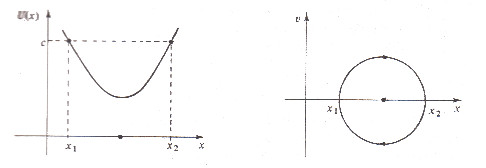
\includegraphics{imagenes/dibu4.jpg}

\item Supongamos $F(x)\neq 0$ para $0<|x-x_0|<a$. Demostrar que
\eqref{conservativo} tiene un centro o una silla en $(x_0,0)$
acorde a $U(x_0)$ sea un m'inimo o un m'aximo relativo.

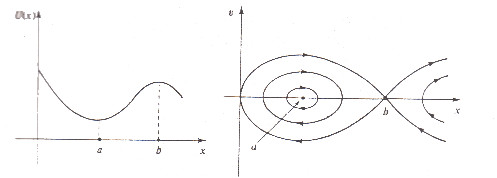
\includegraphics{imagenes/dibu5.jpg}
\end{enumerate}


\end{ejercicio}

\begin{ejercicio}{} Utilizando el ejercicio anterior determinar el
espacio de fases de las siguientes ecuaciones:
\begin{enumerate}
\item $x''=-x$ (resorte).
\item $x''=-\hbox{sen } x$ (p'endulo).
\item $x''=-\frac{1}{x^2}$ (gravitaci'on).
\end{enumerate}
\end{ejercicio}





\begin{ejercicio}{} Sea $f:D\to\mathbb{R}^n$ una campo vectorial
continuo. Una funci'on $E:D\to\mathbb{R}$ se llama integral
primera de $f$ en $D$ si:
\begin{enumerate}
\item $E$ es constante sobre cada 'orbita de $f$.
\item $E$ no es constante en ning'un subconjunto abierto de $D$.

\end{enumerate}
Resolver los siguientes problemas:
\begin{enumerate}
\item Sea $E:D\to\mathbb{R}$  de clase
$C^1$  tal que
\[
    DE(x).f(x)=0\quad\hbox{y}\quad DE(x)\neq 0,
\]
para todo $x$, donde $DE$ denota el diferencial de $E$. Entonces
$E$ es una integral primera.
\item Encontrar una integral primera para el centro dado por:
\[
    \left\{%
\begin{array}{ll}
   x_1'=-\beta x_2 \\
    x_2'=\beta x_1 \\
\end{array}%
\right.
\]
y de la silla
\[
    \left\{%
\begin{array}{ll}
   x_1'=\lambda_1 x_1 \\
    x_2'=\lambda_2 x_2 \\
\end{array}%
\right.
\]
donde $\lambda_1<0<\lambda_2$.

\item Demostrar que no existe una integral primera para los
sumideros o fuentes lineales en $\mathbb{R}^2$.

\item Generalizar los dos incisos anteriores a
sistemas lineales en $\mathbb{R}^n$.

\item Sea $H:\mathbb{R}^{2n}\to\mathbb{R}$ una funci'on de clase
$C^1$. Supongamos que los puntos donde $DH(x)=0$ son aislados.
Encontrar una integral primera para el campo:
\[
    f(x_1,\ldots,x_{2n})= \bigg(\frac{\partial H}{\partial
    x_{n+1}},\ldots, \frac{\partial H}{\partial x_{2n}},
    -\frac{\partial H}{\partial x_{1}},\ldots,
    -\frac{\partial H}{\partial x_{n}} \bigg).
\]
Tal campo se lo conoce como Hamiltoniano.

\item Sea $D\subset\mathbb{R}^2$ y $E:D\to\mathbb{R}$  de clase
$C^1$ tal que $DE$ no se anula en ning'un abierto de $D$.
Encontrar un campo $f$ que tenga a $E$ por integral primera.


\item Demostrar que si $E$ es una integral primera de $f$ entonces
$M_c=f^{-1}(c)$ es invariante para el flujo generado por $f$. En
particular podemos considerar las 'orbitas contenidas en $M_c$
como un ``subsistema'' de una dimensi'on menor en una unidad al
original.



\end{enumerate}


\end{ejercicio}


\begin{ejercicio}{} Consideremos las ecuaciones de Lotka-Volterra:
\[
    \left\{%
\begin{array}{ll}
    x'=\alpha x-\beta x y\\
    y'=-\gamma x + \delta x y\\
\end{array}%
\right.
\]
donde $\alpha, \beta,\gamma$ y $ \delta$ son positivos. Demostrar
que el sistema tiene una integral primera $E$ que posee en
$(\gamma/\delta, \alpha/\beta)$
 un punto de m'inimo no degenerado (esto es $D^2E$ es definida
 positiva en ese punto). Conclu'ir que todas las soluciones en el
 cuadrante positivo son peri'odicas. \emph{Sugerencia:}
 Transformar el sistema en una ecuaci'on en variables separadas y
 deducir que
 \[
    E=-y^{\alpha}x^{\gamma}e^{-\beta y}e^{-\delta x}
 \]
\end{ejercicio}
\begin{ejercicio}{} Demostrar que el origen es un punto de
equilibrio asint'oticamente estable de:
\[
    \left\{%
\begin{array}{ll}
    x'=-x-\frac{x^3}{3}-2\hbox{sen }y \\
    y'=-y-\frac{y^3}{3}\\
\end{array}%
\right.
\]

\end{ejercicio}

\begin{ejercicio}{} Sea $f:\mathbb{R}^n\to\mathbb{R}$ continua y
supongamos que $f(0)=0$ y $\langle x,f(x)\rangle<0$ $\forall x\neq
0$. Demostrar que $x\mapsto |x|^2$ es una funci'on de Liapunov
estricta para el sistema $x'=f(x)$.

\end{ejercicio}

\begin{ejercicio}{}
Sea $x_0$ un punto de equilibrio de $x'=f(x)$,
$f:D\to\mathbb{R}^n$ continua, $D\subset\mathbb{R}^n$ abierto. Sea
$V:U\to\mathbb{R}$ una funci'on de Liapunov en $x_0$. Supongamos
que no existe una trayectoria del sistema completamente contenida
en $Z:=\{x\in U:\dot{V}=0\}$, excepto $x(t)\equiv x_0$. Entonces
$x_0$ es asintoticamente estable.

\end{ejercicio}


\begin{ejercicio}{}
Sea $x_0$ un punto de equilibrio de $x'=f(x)$,
 $f:D\to\mathbb{R}^n$ continua, $D\subset\mathbb{R}^n$ abierto.
 Sea $V$ una funci'on de clase $C^1$ definida en un entorno de
 $x_0$ tal que $\dot{V}>0$ $\forall x\neq x_0$ y $V(x_0)=0$. Si en
 todo entorno de $x_0$ existe un $x$ tal que $V(x)>0$, entonces
 $x_0$ es inestable.

\end{ejercicio}

\begin{ejercicio}{}
Sea $x_0$ un punto de equilibrio de $x'=f(x)$,
$f:D\to\mathbb{R}^n$ continua, $D\subset\mathbb{R}^n$ abierto. Sea
$V:U\to\mathbb{R}$ una funci'on de Liapunov estricta de $x_0$.
Entonces, para cada $c>0$ tal que $V^{-1}([0,c])$ es compacto se
tiene que $V^{-1}([0,c])\subset E(x_0)$ la variedad estable de
$x_0$.

\end{ejercicio}

\begin{ejercicio}{} Sea $D\subset\mathbb{R}^n$ abierto y
$V:D\to\mathbb{R}$ una funci'on de clase $C^1$. Consideremos el
sistema
\[
    x'=-\nabla V(x).
\]
Demostrar que
\begin{enumerate}
    \item   $\dot{V}(x)\leq 0$ $\forall x\in D$ y $\dot{V}(x)=0$
    si, y s'olo si, $x$ es un punto de equilibrio de $-\nabla
    V$.
    \item Si $x_0$ es un m'inimo aislado de $V$, entonces $x_0$ es
    un punto de equilibrio asint'oticamente estable de $-\nabla V$.
    \item $-\nabla V$ no posee 'orbitas peri'odicas no constantes.
\end{enumerate}
\end{ejercicio}

\begin{ejercicio}{} Sea $V:D\to\mathbb{R}$ una funci'on $C^1$, con
$D\subset\mathbb{R}^n$ abierto. Sea $y$ un punto $\omega$-l'imite
de una trayectoria del campo $-\nabla V$. Entonces $y$ es un punto
 de equilibrio de este campo. \emph{Sugerencia:} Demostrar que $V$
 es constante en $\Omega[x]$ $\forall x$.

\end{ejercicio}

\begin{ejercicio}{} Considerar una part'icula moviendos'e bajo la
influencia de una funci'on potencial $P:D\to\mathbb{R}$ de clase
$C^1$, $D\subset\mathbb{R}^3$ abierto. El sistema din'amico
correspondiente es:
\[
    \left\{%
\begin{array}{ll}
   x'=v, \\
    v'=-\nabla P(x) \\
\end{array}%
\right.
\]
Demostrar el Teorema de Lagrange, seg'un el cual un punto de
equilibrio $(x_0,0)$ del sistema es estable si $x_0$ es un m'inimo
local estricto de $P$.
\end{ejercicio}

\begin{ejercicio}{} Sea $f:\mathbb{R}^n\to\mathbb{R}^n$ tal que
$f(0)=0$. La soluci'on $0$ de $x'=f(x)$ se dice globalmente
estable cuando es estable y $x(t)\to 0$ para $t\to\infty$ para
toda otra soluci'on $x(t)$. Sea $V:\mathbb{R}^n\to\mathbb{R}$ una
funci'on de Liapunov estricta de $x'=f(x)$ en $0$. Supongamos que
para cada $c>0$ existe un $R>0$ tal que $|x|>R$, implica $V(x)>c$.
Entonces $0$ es una soluci'on globalmente estable de $x'=f(x)$.
Observar que no es necesaria la condici'on $V(x)=0$ sii $x=0$. Es
suficiente suponer que no existe una soluci'on $x(t)$, distinta de
la nula, tal que $V(x(t))=0$ $\forall t$.

\end{ejercicio}